\chapter{Lie groups and Lie algebras}
In this chapter, there will be introduced some general concepts about properties of Lie algebras and groups, and their unitary representations, while on the other hand there will be a special focus on the irreducible representations of the $\sua(N)$ Lie algebras and of the corresponding $SU(N)$ Lie groups. This is motivated in part by particle physics, since the Standard Model is based on the $U(1) \times SU(2) \times SU(3)$ gauge symmetry with various proposed extension involving higher-dimensional $SU(N)$ groups. In addition, $SU(N)$ Lie groups also have important applications in condensed matter theory and other areas of physics. 

First, the definition of a Lie group is recalled, though in a more precise way.
\begin{defn}[Lie group]
    A Lie group $G$ is a differentiable manifold with a group internal operation $\cdot : G \times G \to G$, $(g,g') \mapsto g'' \in G$ for any $g,g' \in G$, such that:
    \begin{enumerate}
        \item is associative, namely $g\cdot(g'\cdot g'') = (g\cdot g')\cdot g''$, for any $g,g',g'' \in G$;
        \item there exists a unit element $e \in G$ such that $e\cdot g = g\cdot e = g$ for every $g \in G$;
        \item there exists an inverse element $g^{-1} \in G$ such that $g^{-1}\cdot g = g\cdot g^{-1} = e$ for every $g \in G$;
        \item is smooth to guarantee that the multiplication and inverse operation are also smooth, namely that requires the smoothness of the map $(g,g') \mapsto g^{-1}g'$ for any $g,g' \in G$.
    \end{enumerate}
\end{defn}
\begin{defn}[Lie subgroup]
    A subgroup $H$ of a Lie group $G$ is a Lie subgroup if the inclusion map $i : H \to G$, $i(h) = h$ is an injective immersion, namely an embedding of $H$ into $G$ as a submanifold, and a group homomorphism.
\end{defn}
Examples of Lie groups were already previously encountered, namely the matrix Lie groups $GL(n,\R)$ and $GL(n,\C)$, and their subgroups $SL(n,\R)$, $SL(n,\C)$, $O(n)$, $U(n)$, $SO(n,\R)$ and $SU(n)$. However, the focus will be narrowed to compact Lie groups, whose set contains the $U(1)$, $O(n)$, $SO(n)$, $U(n)$, $SU(n)$ and $Sp(n)$ groups, the compact forms of the exceptional Lie groups $\G_2$, $\F_4$, $\E_6$, $\E_7$ and $\E_8$, and all of their finite direct product groups. For clearness, a compact Lie group is one that is closed and limited. To define a Lie algebra it is necessary to first define what is an algebra. 
\begin{defn}[algebra]
    An algebra is a vector space $V$ over a field $K$ which also has an internal operation $\cdot : V \times V \to V$ that for every element $X,Y,Z \in V$ and $a,b,c \in K$ satisfies the following properties:
    \begin{enumerate}
        \item left distributivity, namely $(aX + bY)\cdot Z = a(X \cdot Z) + b(Y\cdot Z)$;
        \item right distributivity, namely $X \cdot (aY + bZ) = a(X\cdot Y) + b(X \cdot Z)$;
        \item compatibility with scalars, namely $(aX)\cdot(bY) = (ab)(X \cdot Y)$.
    \end{enumerate}
\end{defn}
Then, a Lie algebra is an algebra that satisfies some additional requirements.
\begin{defn}[Lie algebra]
    A Lie algebra is an algebra over a field $K$ equipped with the internal operation $\comm{\dots}{\dots} : V \times V \to V$, called the Lie bracket, which for every element $X,Y,Z \in V$ and $a,b,c \in K$ satisfies the following properties:
    \begin{enumerate}
        \item linearity in the first argument, namely $\comm{aX + bY}{Z} = a\comm{X}{Z} + b\comm{Y}{Z}$;
        \item antisymmetric, namely $\comm{X}{Y} = - \comm{Y}{X}$;
        \item it satisfies the Jacobi identity $\comm{X}{\comm{Y}{Z}} + \comm{Y}{\comm{Z}{C}} + \comm{Z}{\comm{X}{Y}} = 0$.
    \end{enumerate}
\end{defn}
Note that the first two statements of the Lie algebra definition imply linearity also in the second argument, making the Lie algebra bilinear just like the general definition of an algebra require.
\begin{defn}[Abelian Lie algebra]
    A Lie algebra is said to be Abelian if the Lie bracket is commutative, namely if $\comm{X}{Y} = 0$ for any $X,Y \in V$.
\end{defn}
There are other useful definitions that regard subspaces of the vector space $V$.
\begin{defn}[Lie subalgebra]
    If a subspace $W \subset V$ is closed under the Lie bracket, namely if $\comm{X}{Y} \in W$ for any $X,Y \in W$, it is a Lie subalgebra of $V$.
\end{defn}
\begin{defn}[ideal]
    If $\comm{X}{Y} \in W$ for every element $X \in W \subseteq V$ and every element $Y \in V$, then $W \subseteq V$ is called an ideal, or an invariant Lie subalgebra.
\end{defn}
Note that $W = V$ and $W = \{\vo\}$ are always ideals, for this they are called trivial ideals. Conversely, a non-trivial ideal is an ideal that is a proper subset of $V$. The possible existence of non-trivial ideals leads to the introduction of the two following definitions.
\begin{defn}[simple Lie algebra]
    A Lie algebra is said to be simple if it has no non-trivial ideals.
\end{defn}
\begin{defn}[semi-simple Lie algebra]
    A Lie algebra is said to be semi-simple if it has no non-trivial Abelian ideals.
\end{defn}
From these definitions, it follows that all simple Lie algebras are also semi-simple, while the converse statement is not true. In general, semi-simple algebras are direct sums of simple ones. 

To define a Lie algebra, a vector space is first needed. Since a Lie group $G$ is a smooth manifold, one can use the space of vector fields on $G$. However, it will be added one powerful requirement and restrict to a specific set of vector fields. Consider now a manifold $M$ and curve $\curve$ on said manifold, defined as $\curve(t) : (a,b) \to M$ with $t \in (a,b) \subseteq \R$ where it assumed that $0 \in (a,b)$. 
\begin{figure}[h]
    \centering
    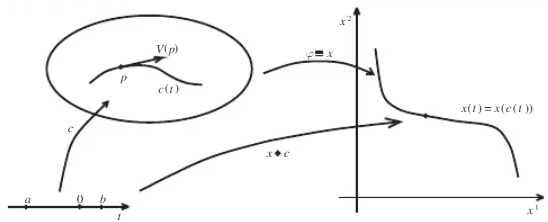
\includegraphics[width=0.7\linewidth]{Immagini - Capitolo 3/curve on manifold.png}
    \caption{a curve $\curve(t)$ on and a tangent vector $v_P$ at $P = \curve(0)$.}
    \label{fig: curve on manifold}
\end{figure}
Let $P \in M$ be a point on the manifold set to be $P \equiv \curve(0)$, and define the vector $v_P$ that is tangent to the curve $\curve$ in the point $P$, namely the tangent vector in a point $P$ of a manifold $M$, as
\begin{equation}
\label{eq: tangent vector on a manifold}
    v_P := v^\mu(P)\frac{\p}{\p x^\mu} = \frac{d}{dt}x^\mu[\curve(t)]\bigg|_{t = 0}\frac{\p}{\p x^\mu}.
\end{equation}
If one defines the function $f : M \to \R$, then, with the previous definition in \eqref{eq: tangent vector on a manifold}, the change in $f$ along the curve $\curve$ can be expressed as
\begin{equation}
    \frac{df}{dt} \equiv v_P[f] = \frac{d}{dt}x^\mu[\curve(t)]\bigg|_{t = 0}\frac{\p f}{\p x^\mu},
\end{equation}
which is precisely the total derivative of $f$ computed along the curve $\curve$. From the definition in \eqref{eq: tangent vector on a manifold}, it follows the next definition.
\begin{defn}[tangent vector space]
    The tangent vectors space $T_PM$ is defined as the set of all tangent vectors $v_P$, and all the possible linear combinations, in a point $P$ of a manifold $M$.
\end{defn}
Since the notion of a dual vector space is understood, it is possible to give the following definition.
\begin{defn}[dual tangent vectors space]
    The dual tangent vectors space $T^*_PM$, also called the cotangent vector space, is the dual vector space of $T_PM$ and it is defined as the set of all linear functions from $T_PM$ to $\R$.
\end{defn}
Consider now two manifolds $M$ and $N$, define a function $f : M \to N$ and let $P$ be a point on $M$, with image $f(P)$ as a point on $N$, as shown in figure \ref{fig: pushforward}, one can define the vector spaces $T_PM$ and $T_{f(P)}M$. Furthermore, given a function $g : N \to \R$, one can construct the composite function $g \circ f : M \to \R$ and ask how this function changes along a curve having $v$ as the tangent vector in $P \in M$. The answer is given by defining the push-forward of $f$ of said tangent vector as 
\begin{equation}
    (f_*v)[g] = v[g \circ f].
\end{equation}
In other words, if $v$ is a tangent vector of a curve $\curve(t)$, so that $v[g \circ f]$ characterises the rate of change of a function $g \circ f$ along the curve $\curve(t)$, then $f_*v$ characterises the rate of change of the function $g$ along the image curve $f(\curve(t))$. The components of the push-forward are
\begin{equation}
    (f_*v)^\nu = v^\mu\frac{\p y(x^\nu)}{\p x^\mu},\quad y^\mu(x^\nu) \equiv f(x^\nu(\curve(t))).
\end{equation}
\begin{figure}[h]
    \centering
    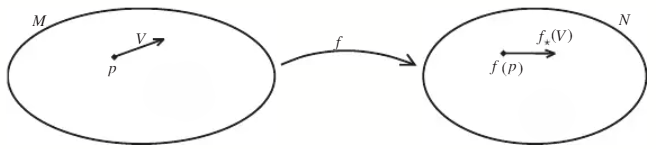
\includegraphics[width=0.7\linewidth]{Immagini - Capitolo 3/pushforward.png}
    \caption{push-forward $f_*v$ of a tangent vector $v \in T_PM$.}
    \label{fig: pushforward}
\end{figure}

Given an element $a \in G$ of a Lie group $G$, one can define the left action as the left translation $L_a : G \to G$, $g \mapsto L_a(g) = a\cdot g$, which is a diffeomorphism\footnote{Since the product must be a smooth map and one of its elements is fixed.}. Then one is going to use the associated push-forward $(L_a)_*$, which maps a tangent vector at $g$ to a tangent vector at $a \cdot g$. In general, given a vector field $X$ on $G$, one could look at its values at points $g$ and $a \cdot g$ to obtain two tangent vectors, however in general these two have no simple relation. Requiring that $X|_g$ is related to $X|_{a\cdot g}$ by the push-forward map, the following definition can be stated.
\begin{defn}[invariant vector field]
    A vector field $X$ on a group $G$ is left-invariant if $(L_a)_* : T_gG \to T_{a\cdot g}G$ satisfies the following condition 
    \begin{equation}
        (L_a)_*X|_g = X|_{a\cdot g}.
    \end{equation}
\end{defn}
This definition can be extended to Lie algebras.
\begin{defn}[invariant Lie algebra]
    A Lie algebra is defined as the set of left-invariant vector fields $\algebra$ on the group $G$ with the commutator defined as 
    \begin{equation}
        \comm{X}{Y} := XY - YX,
    \end{equation}
    where $X$ and $Y$ are vector fields on $G$.
\end{defn}
The set $\algebra$ is a vector space, since the push-forward $(L_g)_*$ is a linear map, and is isomorphic to $T_eG$, hence its dimension is $\dim{\algebra} = \dim{G}$. Since $\algebra$ is also a collector of fields, their commutators can be computed; the result is again left-invariant
\begin{equation}
    (L_a)_*\comm{X}{Y}|_g = \comm{(L_a)_*X|g}{(L_a)_*Y|_g}.
\end{equation}
In turn, using left-invariance, one has $\comm{(L_a)_*X|g}{(L_a)_*Y|_g} = \comm{X|_{a\cdot g}}{Y|_{a\cdot g}}$, hence 
\begin{equation}
    (L_a)_*\comm{X}{Y}|_g = \comm{X|_{a\cdot g}}{Y|_{a\cdot g}} \equiv \comm{X}{Y}|_{a\cdot g}.
\end{equation}
Thus, if $X$ and $Y$ are two arbitrary elements of $\algebra$, then also $\comm{X}{Y}$ is an element of $\algebra$. It is now justified to define a Lie algebra in the following way.
\begin{defn}[Lie algebra]
    A Lie algebra of a Lie group $G$ is the set of left-invariant vector fields $\algebra$ with the commutator $\comm{\dots}{\dots} : \algebra \times \algebra \to \algebra$, $(X,Y) \mapsto \comm{X}{Y}$.
\end{defn}
Note that since $\algebra$ is isomorphic to the tangent space of the Lie group at the identity $T_eG$, it is also justified to consider the latter as the Lie algebra associated with the Lie group. Recall also that in equation \eqref{eq: tangent vector on a manifold} the tangent vector $v$ was defined as an operator associated with a curve $\curve(t)$, or an equivalence class of curves giving the same tangent vector, at a point $P \equiv \curve(0)$, and there was a one-to-one correspondence between equivalence classes of curves and tangent vectors. This definition is useful to find the Lie algebras associated with some matrix Lie groups. For this purpose, it is useful to introduce the following identity 
\begin{equation}
\label{eq: positive matrix identity}
    \det{M} = \exp{(\tr{\ln{M}})},
\end{equation}
for a positive definite matrix $M$, so 
\begin{equation}
    \begin{split}
        \det{(\MI_n + A)} = \exp{[\tr{\ln{(\MI_n + A)}}]} &\simeq \exp{\bigg[\tr{\bigg(A - \frac{A^2}{2} + \cdots \bigg)}\bigg]} \\
        &\simeq 1 + \tr{A} + \cdots.
    \end{split}
\end{equation}
\begin{ex}
    If the Lie algebra is identified with the tangent space at unity, one can construct the Lie algebras of common matrix groups:
    \begin{enumerate}
        \item for $\gla(n,\R)$, it is immediate to get $\gla(n,\R) = \{A \in \R^{n,n}\} \equiv \R^{n,n}$;
        \item for $\sla(n,\R)$, consider a curve $\curve(t)$ that passes through the unit element $e = \MI_n \in SL(n,\R)$ with $e \equiv \curve(0)$ and derive the tangent vector at $t = 0$, thus for small $t$ the curve can be approximated as $\curve(t) \simeq \MI_n + tA + \cdots$, so the tangent vector is found to be
        \begin{equation}
            \frac{d\curve(t)}{dt}\bigg|_{t = 0} = A \in T_eSL(n,\R),
        \end{equation}
        so now by using the relation \eqref{eq: positive matrix identity} and the unit determinant condition one can write
        \begin{equation}
            1 = \det{\curve(t)} = \det{(\MI_n + A)} \simeq 1 + t\tr{A} + \cdots,
        \end{equation}
        thus resulting in $\tr{A} = 0$ and identifying 
        \begin{equation}
            \sla(n,\R) = \{A \in \R^{n,n} : \tr{A} = 0\};
        \end{equation}
        \item for $\soa(n)$, consider a curve $\curve(t) = \MI_n + tA$ and require it to be orthogonal 
        \begin{equation}
            \MI_n = \curve(t)\curve(t)^T = (\MI_n + tA)(\MI_n + tA)^T = \MI + t(A + A^T) + o(t^2),
        \end{equation}
        thus resulting in $A = -A^T$, so one can identify the $\soa(n)$ algebra as the set of antisymmetric real matrices
        \begin{equation}
            \soa(n) = \{A \in \R^{n,n} : A = -A^T\};
        \end{equation}
        \item for $\ua(n)$, consider the curve $\curve(t) = \MI_n + tA$ and impose the unitarity condition
        \begin{equation}
            \MI_n = \curve(t)\curve(t)^\dg = (\MI_n + tA)(\MI_n + tA)^\dg = \MI + t(A + A^\dg) + o(t^2),
        \end{equation}
        to find the constraint $A = -A^\dg$, hence $\ua(n)$ can be identified with the set of anti-Hermitian complex matrices; however in Physics, since in quantum mechanics the observable correspond to Hermitian operators, is more frequent to use the convention in which $t$ is multiplied by the imaginary unit, so by using the curve $\curve(t) = \MI_n + itA$ that leads to the constraint $A = A^\dg$, resulting in the identification
        \begin{equation}
            \ua(n) = \{A \in \C^{n,n} : A = A^\dg\};
        \end{equation}
        \item for $\sua(n)$, imposing the unitarity and the unit determinant conditions, using physics conventions, results in the identification
        \begin{equation}
            \sua(n) = \{A \in \C^{n,n} : A = A^\dg,\,\tr{A} = 0\}.
        \end{equation}
    \end{enumerate}
\end{ex}
Conversely, one can construct elements of the group from elements of the associated algebra using the exponential map, defined as the mapping from a Lie algebra $\algebra$ to the associated Lie group $G$ through
\begin{equation}
    \exp : \algebra \to G,\quad X \mapsto \exp{(X)} \equiv e^X.
\end{equation}
Let $\dim{\algebra} = \dim{G} = n$. Since the Lie algebra is also a vector space, one can choose a basis $\basis_\algebra = \{X_1,\dots,X_n\}$ and expand any element $X \in \algebra$ in this basis as $X = \alpha_aX^a$, where $\alpha_a \in \R$, then using the exponential map 
\begin{equation}
    \exp{(X)} = e^{\alpha_aX^a},
\end{equation}
and varying the parameters $\alpha_a$ a subset $U$ of elements of the Lie group around the unit element $e \in U$ is clearly obtained. Moreover, within $U$, one can use the Baker-Campbell-Hausdorff relation, which states that
\begin{equation}
    e^Xe^Y = \exp{\bigg(X + Y + \frac{1}{2}\comm{X}{Y} + \frac{1}{2}(\comm{X}{\comm{X}{Y}} + \comm{Y}{\comm{Y}{X}}) + \cdots\bigg)},
\end{equation}
to construct the product of two group elements $X$ and $Y$. Note that in Physics conventions, one often includes a factor $i$ in the exponent of the exponential map, writing the group elements as $e^{iX} = e^{i\alpha_aX^a}$.

In general, the image $\im(\algebra)$ of the Lie algebra under the exponentiation may be a proper subset of $G$, namely the exponential map may not be a surjection. However, it is a surjection at least in the following two important cases:
\begin{enumerate}
    \item the Lie group $G$ is compact and connected;
    \item the Lie group is $G \equiv GL(n,\R)$.
\end{enumerate}
Now, consider again the basis $\basis_\algebra = \{X_1,\dots,X_n\}$. The elements $X_a$ of said basis are called the generators of the Lie algebra; in fact, if the Lie algebra is thought of as the tangent space $T_eG$ and its elements as vectors, one can expand the commutator of a pair of basis vectors in the same basis, namely
\begin{equation}
\label{eq: Lie algebra commutator}
    \comm{X_a}{X_b} = f_{ab}^cX_c,
\end{equation}
with coefficients $f_{ab}^c$. If instead one thinks of the Lie algebra as the space of left-invariant vectors fields, there also exists a basis $\{X_a\}$ and one can expand a commutator in the same basis as in equation \eqref{eq: Lie algebra commutator}. However, now a potential ambiguity could arise. For the vector fields, the $f_{ab}^c$ do not need to be constant numbers. In general, one would expect them to be some smooth functions on the group manifold. If that was the case, there would exists two conflicting interpretations of the Lie algebra. In reality, however, the $f_{ab}^c$ turn out to be constants known as ``structure constants'' of the Lie algebra. Note that the structure constants really define the Lie algebra. Consider the commutator $\comm{Y}{Z}$ of any pair elements of the algebra, expanding in the basis $\{X_a\}$ the elements $Y = Y^aX_a$ and $Z = Z^aX_a$, where $Y^a$ and $Z^a$ are the components, one gets
\begin{equation}
    \comm{Y}{Z} = Y^aZ^b\comm{X_a}{X_b} = f_{ab}^cY^aZ^aX_c,
\end{equation}
which determines the commutator uniquely, by determining its coefficients. Let $\{V_1,\dots,V_n\}$ be a basis of $T_eG$, assuming $\dim{G} = n < \infty$. Then $\{X_a|_g = (L_g)_*V_a\}$ for $a = 1,\dots,n$, is basis of $T_gG$. Since the vectors $\{V_1,\dots,V_n\}$ are linearly independent, $\{X_1|_g,\dots,X_n|_g\}$ are also linearly independent. The push-forward $(L_g)_*$ is an isomorphism between $T_eG$ and $T_gG$, and $(L_g)_*^{-1} = (L_{g^{-1}})_*$. Since $V_a$ are basis vectors of $T_eG$, one can expand the commutator 
\begin{equation}
    \comm{V_a}{V_b} = f_{ab}^cV_c.
\end{equation}
Let's then push this to $T_gG$; one the one hand
\begin{equation}
    (L_g)_*\comm{V_a}{V_b} = \comm{(L_g)_*V_a}{(L_g)_*V_b} = \comm{X_a|_g}{X_b|_g};
\end{equation}
on the other hand
\begin{equation}
    (L_g)_*(f_{ab}^cV_c) = f_{ab}^cX_c|_g.
\end{equation}
Thus, one obtains 
\begin{equation}
    \comm{X_a|_g}{X_b|_g} = f_{ab}^cX_c|_g.
\end{equation}
Letting $g$ vary over all $G$, one get the same equation everywhere on $G$ with the same numbers $f_{ab}^c$. Thus one can write 
\begin{equation}
    \comm{X_a}{X_b} = f_{ab}^cX_c.
\end{equation}
Note that the antisimmetry of the commutator $\comm{X_a}{X_b} = -\comm{X_b}{X_a}$ implies that the structure constants have the antisimmetry property
\begin{equation}
    f_{ab}^c = -f_{ba}^c.
\end{equation}
Moreover, from the Jacobi identity for the commutator one can also derive the following identity for the structure constants 
\begin{equation}
    f_{ab}^cf_{cd}^e + f_{bd}^cf_{ca}^e + f_{da}^cf_{cb}^e = 0.
\end{equation}
Note that both upper and lower indices have been used, so it is legitimate to ask if one can raise or lower them. It turns out that there is a metric to use for this purpose. However, in the case of semi-simple Lie algebras the metric is the flat Euclidean metric $\delta_{ab}$. Consequently, the placement of the indices does not matter, namely they can be raised and lowered freely. Hence, one can write $f_{ab}^c \equiv f_{abc}$, thus having the structure constants identity written as
\begin{equation}
    f_{abc}f_{cde} + f_{bdc}f_{cae} + f_{dac}f_{cbe} = 0.
\end{equation}

\section{Irreducible representations of Lie algebras}
For finite groups, theorem \ref{teo: reducibility of unitary representations} showed that every finite-dimensional representation is unitary, and theorem \ref{teo: Maschke's theorem} said that all unitary representations are completely reducible. The corresponding statements for compact Lie groups are found in the following two theorems.
\begin{teo}
    All of the finite-dimensional representations of a compact Lie group are equivalent to unitary representations.
\end{teo}
Then, the complete reducibility of unitary representations is stated by the second part of the Peter-Weyl theorem, which is composed of three parts.
\begin{teo}[Peter-Weyl theorem, II part]
    Every unitary representation of a compact group $G$ on a complex Hilbert space is completely reducible, namely it can be fully decomposed into a direct sum of irreducible finite-dimensional unitary representations of $G$.
\end{teo}
There are two important irreducible representations that need to be discussed first. The first one is the defining representation, which is a representation of the underlying abstract group structure using matrices. For example, in the case of the $SU(2)$ Lie group, the three generators $J_a$ are represented by $2 \times 2$ matrices, proportional to the Pauli matrices
\begin{equation}
\label{eq: generators of the SU(2) defining rep}
    \bigg\{J_1 = \frac{1}{2}
    \begin{pmatrix}
        0 & 1 \\
        1 & 0
    \end{pmatrix},\,
    J_2 = \frac{1}{2}
    \begin{pmatrix}
        0 & -i \\
        i & 0
    \end{pmatrix},\,
    J_1 = \frac{1}{2}
    \begin{pmatrix}
        1 & 0 \\
        0 & -1
    \end{pmatrix}\bigg\}.
\end{equation}
It should be remarked that there is an arbitrariness involved in the choice of the normalisation of the generators, so the defining representation is not unique. The choice made in \eqref{eq: generators of the SU(2) defining rep} is the choice of a defining representation of $\sua(2)$ for which the structure constants are defined as $f_{abc} = \epsilon_{abc}$. The dimension $m$ of the defining representation is usually not the same as the dimension $N$ of the Lie group and Lie algebra. However, that is the case for the second important irreducible representation, the adjoint representation. Given a basis $\basis_\algebra = \{X_a\}$ of $\algebra$, the group elements $g$ are represented in the adjoint representation $D^{adj}$, with $\dim{D^{adj}} = \dim{\algebra}$, by the matrices $D^{adj}(g)$ whose action from the right is defined as
\begin{equation}
    gX_ag^{-1} = X_b[D^{adj}(g)]^b_a.
\end{equation}
Furthermore, using the structure constants $f_{abc}$ one has
\begin{equation}
  \comm{X_a}{X_b} = if_{abc}X_c,
\end{equation}
so from the comparison of the latter two equations, one can introduce a matrix $D^{adj}(X_a)$ with the components $[D^{adj}(X_a)]_{bc} = -if_{abc}$. In the end the adjoint representation of the Lie algebra means simply representing the generators $X_a$ with the $N \times N$ matrices $D^{adj}(X_a)$. Note also that since the matrix elements are defined by the structure constants, which depends on the choice of basis, there is some ambiguity and in particular there exists a preferred choice of basis, but in this context is not really relevant.

\subsection{Dynkin index, Casimir operators and anomalies}
Assume that $D$ is a finite-dimensional representation of an algebra $\algebra$ with $\dim{\algebra} = N$, where the $N$ generators $X_a$ are matrices. 
\begin{notz}
    From now on, it is used $X_a$ in place of $D(X_a)$ for a shorter notation.
\end{notz}
One can define a $N \times N$ matrix $M$ with elements $M_{ab} = \tr{(X_aX_b)}$. Said matrix is symmetric and real, so one can diagonalise it by an orthogonal matrix $O$ such that 
\begin{equation}
    M' = OMO^T,
\end{equation}
where $M'$ is indeed diagonal, and move to a new basis of generators $X_a' = (OX)_a$. The eigenvalues of $M'$ are real. For the non-zero ones, one can do a further rescaling of the corresponding generator $X_a' \to rX_a'$ with $r \in \R\setminus\{0\}$; this will rescale $\lambda_a \to r^2\lambda_a$ without changing its sign. In the case of semi-simple Lie groups and algebras, all $\lambda_a$ will be positive, so by rescaling the generators it possible to adjust them to the same positive value $\lambda_D$. In other words, one can choose a basis of generators where
\begin{equation}
    \tr{(X_aX_b)} = \lambda_D\delta_{ab},\quad \lambda_D > 0.
\end{equation}
An important note, is that the numerical value of $\lambda_D$ is not independent on the particular representation $D$, as different representations involve different matrices of different size, which has an effect on the trace, and the basis of generators together with the possibility to rescale them are already fixed. The number $\lambda_D$ is called the ``Dynkin index'' of the representation $D$. For the direct-sum representation $D_1 \op D_2$ the Dynkin index satisfies the relation
\begin{equation}
\label{eq: Dynkin index of direct sum}
    \lambda_{D_1 \op D_2} = \lambda_{D_1} + \lambda_{D_2},
\end{equation}
while the tensor-product representation $D_1 \ot D_2$ it satisfies
\begin{equation}
\label{eq: Dynkin index of tensor product}
    \lambda_{D_1 \ot D_2} = (\dim{D_1})\lambda_{D_2} + (\dim{D_2})\lambda_{D_1}.
\end{equation}
Another important quantity is the second-order Casimir operator $C^{(2)}$ defined as
\begin{equation}
    C^{(2)} = \sum_{a=1}^NX_aX_a \equiv X_aX^a = X_1^2 + \cdots + X_N^2,
\end{equation}
that has the property to commute with all the generators, namely
\begin{equation}
    \comm{C^{(2)}}{X_a} = 0,\quad \forall a = \{1,\dots,N\},
\end{equation}
and hence with all the elements of the Lie algebra. It turns out that $C^{(2)}$ must be proportional to the identity operator, in particular the proportionality depends on the representation. So, let $D$ be an irreducible representation with $\dim{D} = n$, then in $D$ one has
\begin{equation}
    C^{(2)} = C_2(D)\MI_n,
\end{equation}
where $C_2(D)$ is called the ``quadratic Casimir'' of the representation $D$. Moreover, there exists a relation between the second-order Casimir operator and the Dynkin index, derived as follows
\begin{equation}
    \begin{split}
        \lambda_D\dim{\algebra} = \lambda_D\sum_{a=1}^{\dim{\algebra}}\delta_{aa} &= \sum_{a=1}^{\dim{\algebra}}\tr{(X_aX_a)} \\
        &= \tr{[C^{(2)}]} \\
        &= C_2(D)\tr{(\MI_n)} \\
        &= nC_2(D),
    \end{split}
\end{equation}
thus 
\begin{equation}
    \lambda_D = \frac{\dim{D}}{\dim{\algebra}}C_2(D).
\end{equation}
As the name suggests, the definition of a Casimir operator can be generalized to the $n$th order. However, Casimir operator of higher order may be not unique. Nonetheless, it is worthwhile looking at third-order Casimir operator. Let $X_a$ be the generators represented in a choice of defining representation. Define a $(3,0)$-tensor $d_{abc}$ as
\begin{equation}
    d_{abc} = \tr{(\acomm{X_a}{X_b}X_c)},\quad \acomm{X_a}{X_b} = X_aX_b + X_bX_a.
\end{equation}
One can check that $d_{abc}$ is completely symmetric. Then, moving to generators in a generic representation $D$, one finds that
\begin{equation}
\label{eq: anomaly of a representation}
    \tr{[\acomm{D(X_a)}{D(X_b)}D(X_c)]} = A(D)d_{abc}.
\end{equation}
The coefficient $A(D)$ is called the ``anomaly'' of the representation $D$ and it depends on said representation. 
\begin{obs}
    The name ``anomaly'' derives from gauge field theories. Those are theories that are constructed starting from a classical symmetry transformation described by a Lie group, which is ``gauged'' by making the symmetry transformation parameters space-time dependent, namely promoting them to functions. Elementary particles are then described as excitations of quantum fields, which are chose from the irreducible representations of the symmetry group. The invariance of the theory under the symmetry is valid at the classical level, but may be destroyed in the quantisation of the theory, by the regularisation and renormalization processes that are involved. If that happens, then the symmetry is said to be anomalous. For the quantum theory to be well-behaved and consistent, it is crucial that the gauge symmetry holds at the quantum level and does not become anomalous. Typically, checking for the absence of an anomaly can be done by calculations involving equation \eqref{eq: anomaly of a representation}, and it becomes a simple algebraic task to check if an anomaly can be avoided by computing the sum of anomalies of all the involved representations, ans verifying if the total anomaly is zero.  
\end{obs}
Given two representations $D_1$ and $D_2$, the anomaly of their direct sum and tensor product are respectively given by
\begin{align}
    A(D_1 \op D_2) &= A(D_1) + A(D_2), \\
    A(D_1 \ot D_2) &= (\dim{D_1})A(D_2) + (\dim{D_2})A(D_1). 
\end{align}
which are analogous to those of the Dynkin index equations \eqref{eq: Dynkin index of direct sum} and \eqref{eq: Dynkin index of tensor product}. Moreover, anticipating the definition of the complex-conjugate representation $\bar{D}$ of a generic representation $D$ as the one where the generators are represented by the matrices $-X_a^*$, where $X_a$ are the generators of $D$, the anomaly follows the property
\begin{equation}
    A(\bar{D}) = -A(D).
\end{equation}

\section{Roots and weights}
The focus now is on the classification of unitary irreducible representations for a simple or semi-simple Lie algebra $\algebra$ of dimension $\dim{\algebra} = N$. In general, one can find a set of mutually commuting and hence simultaneously diagonalisable generators $\{H_1,\dots,H_m\}$ and classify the irreducible representations by a ``highest'' $m$-component eigenvalue vector $(\mu_1,\dots,\mu_m)$. Then, among all the eigenvalue vectors of the representations, called ``weights'', one can move by ladder operators $E_{\pm\valpha}$, which come in pairs and form the remaining set of generators. The vectors $\pm\valpha$ are called ``roots'' and the operators $E_{\pm\valpha}$ are called ``root generators''. 

Consider a unitary irreducible representation $D$ of $\algebra$. Let $\{X_a\}$ denote the generators of $\algebra$ in the representation $D$. In the vector space spanned by these generators, one searches for the largest set of linear combinations $H_i = \sum_ar_{ia}X_a$, with real coefficients $r_{ia}$, such that $\comm{H_i}{H_j} = 0$ for any $i,j \in \{1,\dots,n\}$. Note that it is always possible to find at least one $H_i$, since it commutes with itself. The reality of the $r_{ia}$ coefficients and the Hermiticity of the $X_a$ generators implies that the $H_i$ are Hermitian too. By a suitable choice of linear combinations and rescalings, one can diagonalise the matrix $\tr{(H_iH_j)}$ and adjust all the eigenvalues to be the same, to arrive at
\begin{equation}
\label{eq: Cartan generators}
    \tr{(H_iH_j)} = k_D\delta_{ij},
\end{equation}
where the coefficient $k_D$ depends on the representations $D$. The $H_i$ generators, satisfying equation \eqref{eq: Cartan generators}, are called the ``Cartan generators'' of the Lie algebra, and their maximal number, often denoted as $m$, is called the ``rank'' of the Lie algebra, or of the associated Lie group. Note that said equation implies that Cartan generators form an Abelian subalgebra of $\algebra$. As a consequence of again equation \eqref{eq: Cartan generators}, the $m$ independent Cartan generators in the given representation $D$ can be diagonalised simultaneously. Since the $H_i$ are Hermitian, their eigenvalues are real numbers noted as $\mu_i$. The corresponding eigenvectors are denoted as $\ket{\vmu,D}$ and are representation specific. The $m$-component vector $\vmu$ is called a ``weight vector'' for that representation. In particular, for the adjoint representation, the weight vectors are also called ``root vectors''. 

Let's choose a basis for $\algebra$, in which the first $m$ basis vectors are precisely the $H_i$ generators, that is, $X_i = H_i$ for $i = \{1,\dots,m\}$. Now consider the adjoint representation, as its dimension is equal to $\dim{\algebra}$, it is possible to build a one-to-one mapping between the generators $X_a$ and the basis vectors of the adjoint representation. The one can use the generators as labels of the basis vectors and denote the latter by $\ket{X_a}$. Furthermore, one can define a scalar product in this space via the Hilbert-Schmidt inner product 
\begin{equation}
    \mybraket{X_a}{X_b} \equiv \tr{(X_a^\dg X_b)} = \tr{(X_a X_b)}.
\end{equation}
Moreover, one can choose the basis such that the generators satisfy 
\begin{equation}
    X_a\ket{X_b} = if_{abc}\ket{X_c},
\end{equation}
where the coefficients $f_{abc}$ are the Lie algebra structure constants. One can adopt a more concise notation
\begin{equation}
    \ket{\comm{X_a}{X_b}} \equiv if_{abc}\ket{X_c},
\end{equation}
so that it is possible to use the commutator as the label of the vector $f_{abc}\ket{X_c}$, and the using the notation
\begin{equation}
    X_a\ket{X_b} = \ket{\comm{X_a}{X_b}}.
\end{equation}
Thus, as a consequence of the condition $\comm{H_i}{H_j} = 0$ one has
\begin{equation}
    H_i\ket{H_j} = 0,\quad \forall i,j \in \{1,\dots,m\}.
\end{equation}
The remaining $n - m$ vectors for $\algebra$ can then be chosen as the other eigenvectors of the $H_i$ generators, denoting them as $\ket{E_{\valpha}}$, where their label $\valpha$ is the list of eigenvalues
\begin{equation}
\label{eq eigenvalue equation of Cartan generators}
    H_i\ket{E_{\valpha}} = \alpha_i\ket{E_{\valpha}}.
\end{equation}
Note that no $\valpha$ can be a null vector, otherwise the corresponding $E_{\valpha}$ would be a Cartan generator itself, in contradiction with the assumption that it is not. Also note that since the Cartan generators are Hermitian, all $\valpha$ are real-component vectors. Now applying $X_a\ket{X_b} = \ket{\comm{X_a}{X_b}}$ to equation \eqref{eq eigenvalue equation of Cartan generators} one has
\begin{equation}
    H_i\ket{E_{\valpha}} = \ket{\comm{H_i}{E_{\valpha}}}.
\end{equation}
In turn, by linearity one can rewrite the right-hand side as $\ket{\alpha_i E_{\valpha}}$, thus one obtains $\ket{\comm{H_i}{E_{\valpha}}} = \ket{\alpha_iE_{\valpha}}$. Equivalently, the latter equation can be rewritten as an equality 
\begin{equation}
    \comm{H_i}{E_{\valpha}} = \alpha_i E_{\valpha},
\end{equation}
which is an algebraic relation, and thus must hold true in all representations. In addition to the fact that all $\valpha$ are real-component vectors, the latter equation implies that the operators $E_{\valpha}$ are non-Hermitian, and that they appear in pairs with opposite eigenvalues $E_{\pm\valpha}$, with $E_{\valpha}^\dg = E_{-\valpha}$.

Now it is interesting to study the effect of the eigenvectors of the Cartan generators $\ket{\vmu,D}$ with one of the $E_{\valpha}$. One can prove that this yields an eigenvector of the Cartan generators with a different eigenvalue
\begin{equation}
    \begin{split}
        H_iE_{\valpha}\ket{\vmu,D} &= \comm{H_i}{E_{\valpha}}\ket{\vmu,D} + E_{\valpha}H_i\ket{\vmu,D} \\
        &= \alpha_iE_{\valpha}\ket{\vmu,D} + \mu_iE_{\valpha}\ket{\vmu,D} \\
        &= (\mu_i + \alpha_i)E_{\valpha}\ket{\vmu,D},
    \end{split}
\end{equation}
which means that $E_{\valpha}\ket{\vmu,D}$ is proportional to the eigenvector of $H_i$ with eigenvalue $(\mu_i + \alpha_i)$, namely
\begin{equation}
\label{eq: Ea on an eigenvector of Hi}
    E_{\valpha}\ket{\vmu,D} = N_{\valpha,\vmu}\ket{\vmu + \valpha,D},
\end{equation}
which holds for every representation $D$, but $N_{\valpha,\vmu}$ depends on $D$. Before determining $N_{\valpha,\vmu}$, consider the adjoint representation, and use the mapping between elements of the algebra and vector states, which implies that $E_{\valpha}\ket{E_{-\valpha}}$ has weight zero, because
\begin{equation}
    \begin{split}
        H_iE_{\valpha}\ket{E_{-\valpha}} &= \comm{H_i}{E_{\valpha}}\ket{E_{-\valpha}} + E_{\valpha}H_i\ket{E_{-\valpha}} \\
        &= \alpha_iE_{\valpha}\ket{E_{-\valpha}} - \alpha_iE_{\valpha}\ket{E_{-\valpha}} \\
        &= 0.
    \end{split}
\end{equation}
This implies that $E_{\valpha}\ket{E_{-\valpha}}$ is a linear combination of the zero-eigenvalue vectors associated with the Cartan subalgebra
\begin{equation}
    E_{\valpha}\ket{E_{-\valpha}} = \sum_{i=1}^m c_i\ket{H_i}.
\end{equation}
It turns out, since in the adjoint representation the generators are normalised as $\tr{(X_aX_b)} = \lambda\delta_{ab}$, that $c_i = \alpha_i$, thus $E_{\valpha}\ket{E_{-\valpha}} = \sum_{i=1}^m \alpha_i\ket{H_i}$, or equivalently
\begin{equation}
    \ket{\comm{E_{\valpha}}{E_{-\valpha}}} = \sum_{i=1}^m \alpha_i\ket{H_i}.
\end{equation}
From this latter result, it is then straightforward to derive the value of the coefficient $N_{\valpha,\vmu}$; for a generic representation $D$, one has
\begin{equation}
    \mybrakett{\vmu,D}{\comm{E_{\valpha}}{E_{-\valpha}}}{\vmu,D} = \alpha_i\mybrakett{\vmu,D}{H_i}{\vmu,D} = \valpha \cdot \vmu.
\end{equation}
On the other hand, this quantity is also equal to
\begin{equation}
    \begin{split}
        \mybrakett{\vmu,D}{\comm{E_{\valpha}}{E_{-\valpha}}}{\vmu,D} &= \mybrakett{\vmu,D}{E_{\valpha}E_{-\valpha}}{\vmu,D} - \mybrakett{\vmu,D}{E_{-\valpha}E_{\valpha}}{\vmu,D} \\
        &= |N_{-\valpha,\vmu}|^2 - |N_{\valpha,\vmu}|^2,
    \end{split}
\end{equation}
where $N_{-\valpha,\vmu} = N^*_{\valpha,\vmu - \valpha}$, so that 
\begin{equation}
    |N_{-\valpha,\vmu}|^2 - |N_{\valpha,\vmu}|^2 = \valpha \cdot \vmu.
\end{equation}
As remarked above, applying $E_{\valpha}$ to a generic vector $\ket{\vmu,D}$ turns it into a new vector, which is linearly independent from $\ket{\vmu,D}$. If the representation $D$ is finite-dimensional, iterating the procedure cannot generate arbitrarily many linearly independent vectors: there must exist a finite maximum natural number $p$ such that $E_{\valpha}^p\ket{\vmu,D} \propto \ket{\vmu + p\valpha,D}$, but $E_{\valpha}\ket{\vmu + p\valpha,D} = 0$. Thus, $p$ represents the maximum number of times that the raising operator $E_{\valpha}$ can be applied to the vector $\ket{\vmu,D}$, obtaining a linearly independent vector. Note that, in view of equation \eqref{eq: Ea on an eigenvector of Hi}, this means that $N_{\valpha,\vmu + p\valpha} = 0$. Similarly, for the lowering operator $E_{-\valpha}$, there must exist a finite maximum natural number $q$ such that $E_{-\valpha}^q\ket{\vmu,D} \propto \ket{\vmu - q\valpha,D}$, but $E_{-\valpha}\ket{\vmu - q\valpha,D} = 0$, namely $N_{-\valpha,\vmu - q\valpha} = 0$. 

Now consider the relation $|N_{-\valpha,\vmu}|^2 - |N_{\valpha,\vmu}|^2 = \valpha \cdot \vmu$ for $D$, as well for all vectors obtained by applying the $E_{\valpha}$ operator on it once, twice, and so on until the $p$th time, and for those applying the $E_{-\valpha}$ operator once, twice, and so on until the $q$th time. Summing all of these equations together, one obtains
\begin{equation}
    \sum_{k=-q}^p(|N_{\valpha,\vmu + (k - 1)\valpha}|^2 - |N_{\valpha,\vmu + k\valpha}|^2) = \sum_{k=-q}^p\valpha \cdot (\vmu + k\valpha).
\end{equation}
On the left-hand side of the latter equation, the second term of each summand cancels against the first term of the next summand. Thus, the sum reduces to the difference of the first term in the first summand, minus the second term in the last summand, namely to $|N_{\valpha,\vmu - (q + 1)\valpha}|^2 - |N_{\valpha,\vmu + p\valpha}|^2$. As remarked before, however, both of these quantities vanish, so the left-hand of said equation is zero. The right hand side however can be rewritten as
\begin{equation}
    \begin{split}
        \sum_{k=-q}^p\valpha\cdot(\vmu + k\valpha) &= \sum_{k=-q}^p(\valpha\cdot\vmu) + (\valpha \cdot \valpha)\sum_{k=-q}^pk \\
        &= (\valpha \cdot \vmu)(q + p + 1) + (\valpha \cdot \valpha)\frac{(p + q + 1)(p - q)}{2}.
    \end{split}
\end{equation}
Thus, the equation is now 
\begin{equation}
    (\valpha \cdot \vmu)(q + p + 1) + (\valpha \cdot \valpha)\frac{(p + q + 1)(p - q)}{2} = 0,
\end{equation}
by using the fact that $(q + p + 1) > 0$ since both $q$ and $p$ are natural numbers, defining the integer $M \equiv q - p$ and considering that $\valpha \neq \vo$, one remains with
\begin{equation}
    \frac{\valpha \cdot \vbeta}{\alpha^2} = \frac{M}{2},\quad \alpha^2 \equiv  \valpha \cdot \valpha.
\end{equation}
When considering the adjoint representation, the latter equation must hold for any pair of different roots $E_{\valpha}$ and $E_{\vbeta}$, namely equations
\begin{equation}
    \begin{cases}
        \dfrac{\valpha \cdot \vbeta}{\alpha^2} = \dfrac{M}{2} \\[2ex]
        \dfrac{\vbeta \cdot \valpha}{\beta^2} = \dfrac{M'}{2}
    \end{cases},\quad M,M' \in \N.
\end{equation}
must hold simultaneously. Multiplying those two equations together one obtains
\begin{equation}
    \frac{(\valpha \cdot \vbeta)^2}{\alpha^2\beta^2} = \frac{MM'}{4},
\end{equation}
namely, denoting the angle between $\valpha$ and $\vbeta$ as $\theta_{\valpha\vbeta}$, the equation
\begin{equation}
\label{eq: roots Diophantine equation}
    4\cos^2{\theta_{\valpha\vbeta}} = MM'.
\end{equation}
The equation found in \eqref{eq: roots Diophantine equation} is a polynomial equation for which only integer solutions are considered. An equation of this type is called a Diophantine equation. Note that since both $M$ and $M'$ are integers, their product $MM'$ must be an integer itself, moreover $0 \le \cos^2{\theta_{\valpha\vbeta}} \le 1$, so the left-hand side is non-negative and never larger than four. These conditions imply that the only admissible solutions are:
\begin{enumerate}
    \item $MM' = 0$, corresponding to $\theta_{\valpha\vbeta} = \pi/2$;
    \item $MM' = 1$, corresponding to $\theta_{\valpha\vbeta} = \pi/3$ or $\theta_{\valpha\vbeta} = 2\pi/3$;
    \item $MM' = 2$, corresponding to $\theta_{\valpha\vbeta} = \pi/4$ or $\theta_{\valpha\vbeta} = 3\pi/4$;
    \item $MM' = 3$, corresponding to $\theta_{\valpha\vbeta} = \pi/6$ or $\theta_{\valpha\vbeta} = 5\pi/6$;
    \item $MM' = 4$, corresponding to $\theta_{\valpha\vbeta} = 0$ or $\theta_{\valpha\vbeta} = \pi$.
\end{enumerate}
The last case however can be discarded as it would imply that $\valpha$ and $\vbeta$ are proportional to each other, in which case they could not be linearly independent. 
\begin{notz}
    From now on, the notation will be simplified by dropping the bold font for vectors.
\end{notz}

\subsection{Weyl reflections and root systems}
Since the weight $\mu$ and the root $\alpha$ initially chose were arbitrary, one can define a map $s_\alpha$ that associate a weight $\mu$ with a new weight $s_\alpha(\mu)$ as
\begin{equation}
\label{eq: Weyl reflection}
    s_\alpha : \mu \mapsto s_\alpha(\mu) \equiv \mu - \frac{2(\alpha \cdot \mu)}{\alpha^2}\alpha.
\end{equation}
The map defined in \eqref{eq: Weyl reflection} is called a ``Weyl reflection''. The name reflections is not completely unjustified; in fact, in general a reflection of a vector $\vv \in \R^m$ with respect to the hyperplane through the origin perpendicular to the vector $\va$ is defined through the function
\begin{equation}
    s_a(v) := v - \frac{2(a \cdot v)}{a^2}a.
\end{equation}
Thus, equation \eqref{eq: Weyl reflection} defines the reflection of the weight $\mu$ with respect to the hyperplane orthogonal to the root $\alpha$. In particular, since the roots are the non-zero weights in the adjoint representation, one can apply the Weyl reflection map a root to another root, leading to the following definition.
\begin{defn}[root system]
    A root system $\Phi$ is defined as the set of all roots $\alpha$ with the following properties:
    \begin{enumerate}
        \item the roots span the Euclidean vector space $\R^m$;
        \item if $\alpha \in \Phi$, then also $-\alpha \in \Phi$;
        \item the set $\Phi$ is closed under the Weyl reflection map $s_\alpha$ for any $\alpha \in \Phi$;
        \item for all pairs of roots $\alpha,\beta \in \Phi$, the number $2(\alpha \cdot \beta)/\alpha^2$ is an integer.
    \end{enumerate}
\end{defn}
Weyl reflections generate a finite group, which acts faithfully in the root system $\Phi$, called the Weyl group. Furthermore, for every root $\alpha \in \Phi$ one can define a ``coroot'' $\alpha^\vee$ as
\begin{equation}
\label{eq: coroot definition}
    \alpha^\vee := \frac{2\alpha}{\alpha^2}.
\end{equation}
Thus, the number
\begin{equation}
    (\alpha^\vee,\beta) \equiv \frac{2(\alpha \cdot \beta)}{\alpha^2}
\end{equation}
is an integer for every coroot-root pair. Moreover, the coroots form a root system $\Phi^\vee$ called the dual root system.

Consider now a basis $\{H_1,\dots,H_m\}$ for the Cartan subalgebra, and let $\{\mu_1,\dots,\mu_m\}$ be the corresponding weights. For the weight vector $\mu = (\mu_1,\dots,\mu_m)$ there are two common alternative definitions. One may define $\mu$ as a positive weight vector when its first non-zero entry is positive. Conversely, $\mu$ is said to be a negative weight vector when its first entry is negative. Finally, $\mu$ is said to be a zero weight vector if all of its entries are zero. Then one defines a strict order among vectors by introducing an order relation, denoted by $>$, that is defined as follows.
\begin{defn}[order relation]
    Given two weight vectors $\mu$ and $\mu'$, when $\mu - \mu'$ is a positive weight vector the order relation states that $\mu > \mu'$.
\end{defn}
The order relation defined allows one to order all states $\ket{\mu,D}$. For a finite representation, it is then possible to identify the highest weight vector, which is the weight vector that is greater than all others. The highest weight vector is unique and does not depend on the chosen basis $\{H_1,\dots,H_m\}$ for the Cartan subalgebra.

As mentioned above, the non-zero weight vectors of the adjoint representation are called root vectors. The $m$ weight vectors corresponding to the Cartan generators are zero vectors. Thus, there are $\dim{(\algebra)} - m$ root vectors, coming in pairs of opposite elements $\pm \alpha$.
\begin{defn}[simple root]
    A simple root is a positive root vector that can not be written as the sum of two positive roots.
\end{defn}
The latter definition leads to the following lemma.
\begin{lem}[difference of simple roots]
    The difference of any two distinct simple roots is not a root.
\end{lem}
\begin{proof}
    Let $\alpha$ and $\beta$ be two distinct simple roots, $\alpha - \beta$ can not be zero, otherwise one would have $\alpha = \beta$, in contradiction with the assumption stated before. If $\alpha - \beta$ is positive, then $\alpha$ can be written as the sum of two positive roots, $\alpha = (\alpha - \beta) + \beta$, in contradiction with the assumption that $\alpha$ is a simple root. Conversely, if $\beta - \alpha$ id positive, then $\beta$ can be written as the sum of two positive roots, $\beta = (\beta - \alpha) + \alpha$, in contradiction with the assumption that $\beta$ is a simple root.  
\end{proof}
Consider two simple roots $\alpha$ and $\beta$ in the adjoint representation; the previous lemma implies that $\beta - \alpha$ is not a root, thus $E_{-\alpha}\ket{\beta} = 0$. This means that, for this representation and for this choice of roots, one has $q = 0$. Similarly, by interchanging $\alpha$ and $\beta$ one obtains that also the $q$ corresponding to this case vanishes. Accordingly, from equation $(\alpha \cdot \beta)/\alpha^2 = M/2$, one obtains that 
\begin{equation}
    \frac{2(\alpha \cdot \beta)}{\alpha^2} = \frac{2|\alpha||\beta|\cos{\theta_{\alpha\beta}}}{\alpha^2} = \frac{2|\beta|\cos{\theta_{\alpha\beta}}}{|\alpha|} = -p \le 0. 
\end{equation}
As both $|\alpha|$ and $|\beta|$ are positive, this implies that the angle between any pair of simple roots is in the range $\theta_{\alpha\beta} \in [\pi/2, \pi)$. 
\begin{lem}
    Every positive root $\phi$ can be written as a linear combination of simple roots $\alpha$ with non-negative integer coefficients $k_\alpha$, namely
    \begin{equation}
        \phi = \sum_{\substack{all\,simple \\
        roots\,\alpha}} k_\alpha\alpha,\quad k_\alpha \in \N.
    \end{equation}
\end{lem}
The properties of simple roots can be encoded into a matrix called the Cartan matrix. Given a Lie algebra $\algebra$ of rank $m$, the elements of the Cartan matrix $A$ are defined as
\begin{equation}
    A^{ij} = \frac{2(\alpha^i \cdot \alpha^j)}{|\alpha^j|^2}.
\end{equation}
Recalling equation \eqref{eq: coroot definition}, introducing the coroots of simple roots as
\begin{equation}
    a^{j\vee} = \frac{2\alpha^j}{|\alpha^j|^2},
\end{equation}
the elements of the Cartan matrix can be written in a more concise way
\begin{equation}
    A^{ij} = (\alpha^i,\alpha^{j\vee}),
\end{equation}
where $(\dots,\dots)$ denote the scalar product. Without giving a detailed proof, the Cartan matrix has the following properties:
\begin{enumerate}
    \item $A^{ij} \in \Z$, with $A^{ij} < 0$ for any $i \neq j$;
    \item $\det{A} \neq 0$, so $A$ is invertible;
    \item $A^{ii} = 2$ for any $i$;
    \item $A$ is generally not symmetric, but if $A^{ij} = 0$ for any $i$ and $j$, then $A^{ji} = 0$;
    \item the product of two off-diagonal entries that are symmetric under reflection with respect to the main diagonal is a natural number less than four, namely $A^{ij}A^{ji} = \{0,1,2,3\}$ for any $i$ and $j$.
\end{enumerate}
There is also a diagrammatic way to encode the information of the Cartan matrix provided by the Dynkin diagram. Such diagram can be constructed from the Cartan matrix through a set of rules, which are the following:
\begin{enumerate}
    \item draw $m$ open circles, one for each simple root $\alpha^i$;
    \item connect the pair of circles representing the simple roots $\alpha^i$ and $\alpha^j$ with the number of lines given by the corresponding product $A^{ij}A^{ji}$, and to this to all pairs;
    \item in the cases where $A^{ij}A^{ji} = 2$ or $A^{ij}A^{ji} = 3$, if $A^{ij} > A^{ji}$ then fill the circle corresponding to $\alpha^i$ (equivalently, draw an arrow pointing from the circle corresponding to $\alpha^i$ to the one corresponding to $\alpha^j$), while if $A^{ij} > A^{ij}$ fill the circle corresponding to $\alpha^j$ (equivalently, draw an arrow pointing from the circle corresponding to $\alpha^j$ to the one corresponding to $\alpha^i$).
\end{enumerate}
In a Dynkin diagram, the number of lines between two circles is related to the angle between the roots to which the circles correspond; in particular, the number of lines is increasing with the angle. More precisely, one has the cases shown in figure \ref{fig: lines rule Dynkin diagrams}. The filling rule (equivalently, the arrow rule) of Dynkin diagrams reflects the fact that for some Lie algebras, other than $SU(n)$, the simple roots may have different lengths: the filled circle (equivalently, the circle where the arrow starts from) is the one associated with the longer of the two simple roots. 
\begin{figure}[h]
    \centering
    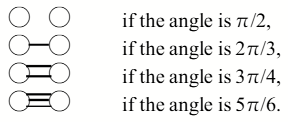
\includegraphics[width=0.4\linewidth]{Immagini - Capitolo 3/lines rule Dynkin diagrams.png}
    \caption{the relation between the number of lines and the angle between two roots in the Dynkin diagrams.}
    \label{fig: lines rule Dynkin diagrams}
\end{figure}
\begin{ex}
    There can be some degenerate diagrams. For example, the Dynkin diagram $\dynkin{C}{2}$ is the same for $C_2$ and $B_2$, this implies that the algebras associated are isomorphic, namely $\soa(6) \simeq \spa(4)$. The same happens for the diagram $\dynkin{D}{3}$ which is shared between $D_3$ and $A_3$, leading to $\soa(6) \simeq \sua(4)$. Instead, the diagram $\dynkin{D}{2}$ of $D_2$ can be written as the ``sum'' of two copies of $A_1$ diagrams $\dynkin{A}{1}$, leading to the relation $\soa(4) \simeq \sua(2) \op \sua(2)$.
\end{ex}
\begin{figure}[h]
    \centering
    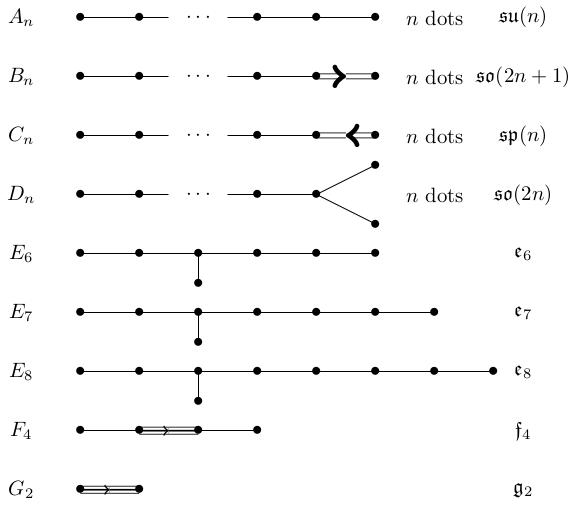
\includegraphics[width=0.5\linewidth]{Immagini - Capitolo 3/finite Dynkin diagrams.png}
    \caption{finite Dynkin diagrams of four infinite families, namely $A_n$, $B_n$, $C_n$ and $D_n$, and of five finite families, namely $g_2$, $f_4$, $e_6$, $e_7$ and $e_8$, with their associated Lie algebras.}
    \label{fig: finite Dynkin diagrams}
\end{figure}
Given an arbitrary irreducible representation $D$, one define a weight vector $\mu$ in $D$ as the highest weight in that representation if and only if, for every positive root $\phi$, the sum $\mu + \phi$ is not a weight in that representation. This is equivalent to requiring that $\mu + \alpha^i$ is not a weight for all simple roots $\alpha^i$. As a consequence, when $E_{\alpha^i}$ acts on $\mu$, the corresponding $p^i$ must be zero, namely equation $(\alpha \cdot \beta)/\alpha^2 = M/2$ must reduce to 
\begin{equation}
    \frac{2(\alpha^i \cdot \mu)}{(\alpha^i)^2} = q^i,\quad q^i \in \N.
\end{equation}
The latter equation can be interpreted as a relation giving the components of $\mu$ on the basis of the simple roots $\alpha^i$. Introducing the coroots of the simple roots by recalling equation \eqref{eq: coroot definition}, this equation can be written in a more concise form
\begin{equation}
    (\alpha^{i\vee},\mu) = q^i.
\end{equation}
Knowing the highest vector $\mu$, one can construct also the other vectors in that representation by acting on $\mu$ with the lowering operators $E_{-\alpha^i}$. This means that every irreducible representation of a simple Lie group of rank $m$ can be uniquely identified by the $m$ natural number $q^i$. It is particularly interesting to consider a set of $m$ irreducible representations $D^i$ with highest vectors $\mu^j$ such that
\begin{equation}
\label{eq: highest vector condition}
    \frac{2(\alpha^i \cdot \mu^j)}{(\alpha^i)^2} = \delta^{ij}.
\end{equation}
Each highest vector satisfying equation \eqref{eq: highest vector condition} is said to be a ``fundamental weight vector''. Using the definition of the coroots of the simple roots given in equation \eqref{eq: coroot definition}, the condition in \eqref{eq: highest vector condition} can be interpreted as an orthonormality relation relation 
\begin{equation}
    (\alpha^{i\vee},\mu^j) = \delta^{ij}.
\end{equation}
Each irreducible representation $D^j$ having a fundamental weight $\mu^j$ as highest vector is said to be a ``fundamental representation''. The fundamental weight provides a basis on which to expand the highest vector of every irreducible representation in a unique way
\begin{equation}
    \mu = \sum_{j=1}^m q^j\mu^j,\quad q^j \in \N.
\end{equation}
Alternatively, one can label the irreducible representation by just listing the integers $(q^1,\dots,q^m)$; this is called the Dynkin label of the representation. With this labelling, the fundamental representations have the labels $(1,0,\dots,0),\dots,(0,\dots,0,1)$.

\section{Lie algebra of SU(3)}
The $SU(3)$ Lie group is defined as the group of $3 \times 3$ complex unitary matrices $U$ having a unit determinant, with matrix multiplication as the group product. The dimension of the associated Lie algebra $\sua(3)$ is $\dim{\sua(3)} = 8$. The generators of $\sua(3)$ are eight Hermitian traceless matrices. A common choice for a defining representation is in terms of a basis given by the Gell-Mann matrices $\lambda_a$, which are the analogue of the Pauli matrices for the algebra of generators of the $SU(2)$ Lie group. The Gell-Mann matrices are
\begin{gather}
    \lambda_1 = 
    \begin{pmatrix}
        0 & 1 & 0 \\
        1 & 0 & 0 \\
        0 & 0 & 0
    \end{pmatrix},\quad 
    \lambda_2 = 
    \begin{pmatrix}
        0 & -i & 0 \\
        i & 0 & 0 \\
        0 & 0 & 0
    \end{pmatrix},\quad 
    \lambda_3 = 
    \begin{pmatrix}
        1 & 0 & 0 \\
        0 & -1 & 0 \\
        0 & 0 & 0
    \end{pmatrix}, \\ 
    \lambda_4 = 
    \begin{pmatrix}
        0 & 0 & 1 \\
        0 & 0 & 0 \\
        1 & 0 & 0
    \end{pmatrix},\quad
    \lambda_5 = 
    \begin{pmatrix}
        0 & 0 & -i \\
        0 & 0 & 0 \\
        i & 0 & 0
    \end{pmatrix},\quad 
    \lambda_6 = 
    \begin{pmatrix}
        0 & 0 & 0 \\
        0 & 0 & 1 \\
        0 & 1 & 0
    \end{pmatrix}, \\ 
    \lambda_7 = 
    \begin{pmatrix}
        0 & 0 & 0 \\
        0 & 0 & -i \\
        0 & i & 0
    \end{pmatrix},\quad 
    \lambda_8 = \frac{1}{\sqrt{3}} 
    \begin{pmatrix}
        1 & 0 & 0 \\
        0 & 1 & 0 \\
        0 & 0 & -2
    \end{pmatrix}.
\end{gather}
The generators $X_a$ of the $\sua(3)$ algebra are then 
\begin{equation}
\label{eq: su(3) algebra generators}
    X_a = \frac{\lambda_a}{2},\quad \forall a = \{1,\dots,8\}.
\end{equation}
The generators are normalised as
\begin{equation}
\label{eq: normalisation of su(3) algebra generators}
    \tr{(X_aX_b)} = \frac{\delta_{ab}}{2},\quad \forall a,b = \{1,\dots,8\},
\end{equation}
so the Dynkin index of the defining representation is 
\begin{equation}
\label{eq: Dynkin index of su(3) algebra defininf representation}
    \lambda_{def.} = \frac{1}{2}. 
\end{equation}
The rank of the $\sua(3)$ algebra is $m = 2$, so in the basis of generators $\{X_a\}$ the generators $X_3$ and $X_8$ are diagonal, thus they are Cartan generators. The often used convention is to name $H_1 \equiv X_3$ and $H_2 \equiv X_8$ as the $\sua(3)$ Cartan generators. Since they are diagonal, their common eigenvectors are
\begin{equation}
    e_1 = 
    \begin{pmatrix}
        1 \\
        0 \\
        0
    \end{pmatrix},\quad
    e_2 = 
    \begin{pmatrix}
        0 \\
        1 \\
        0
    \end{pmatrix},\quad
    e_3 = 
    \begin{pmatrix}
        0 \\
        0 \\
        1
    \end{pmatrix}.
\end{equation}
The eigenvalues of $H_1$ and $H_2$ are the weights $\mu_1$ and $\mu_2$, forming the weight vector $\mu = (\mu_1,\mu_2)$. Moving to the Dirac notation, the weights are used to label the eigenvectors, which are
\begin{equation}
    e_1 = \bigket{\frac{1}{2},\frac{1}{2\sqrt{3}}},\quad e_2 = \bigket{-\frac{1}{2},\frac{1}{2\sqrt{3}}},\quad e_3 = \bigket{0,-\frac{1}{\sqrt{3}}}.
\end{equation}
If one plots the weight vector on the $(\mu_1,\mu_2)$ plane, they form an equilateral triangle, as shown in figure \ref{fig: fundamental and anti-fundamental representation of su(3)}. 
\begin{figure}[h]
    \centering
    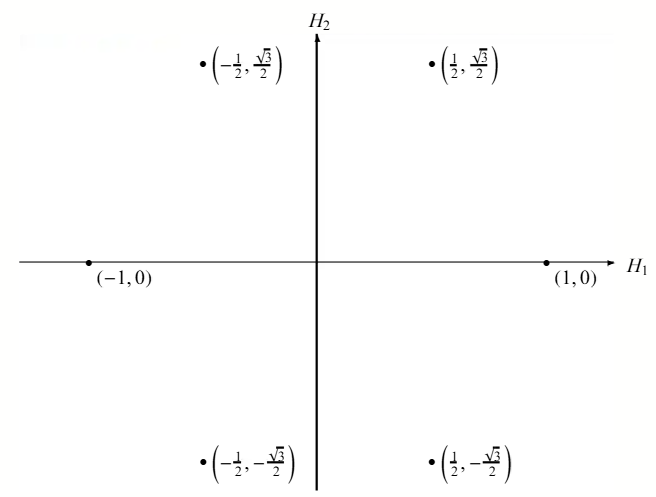
\includegraphics[width=0.55\linewidth]{Immagini - Capitolo 3/roots of su(3).png}
    \caption{roots of the $\sua(3)$.}
    \label{fig: roots of su(3)}
\end{figure}

There will be $8 - 2 = 6$ root vectors, namely three pairs $\pm\alpha$. To find them, one can use the fact that the corresponding generators $E_{\pm\alpha}$ map weights in to one another. Thus, the $\alpha$ vectors are found as differences of weights. In the plot of the weight vectors on the $(\mu_1,\mu_2)$ plane, they correspond to the vectors from one weight to another. Thus, it is simple to read off that the possible $\alpha$ vectors are
\begin{equation}
    \alpha \in \bigg\{ \pm(1,0),\quad \pm\bigg(\frac{1}{2},\frac{\sqrt{3}}{2}\bigg),\quad \pm\bigg(-\frac{1}{2},\frac{\sqrt{3}}{2}\bigg) \bigg\}.
\end{equation}
The roots form a regular hexagon, centred at the origin of the $(H_1,H_2)$ plane, as shown in figure \ref{fig: roots of su(3)}. Note also that all angles between root vectors of the $\sua(3)$ algebra are multiples of $\pi/3$. 
\begin{figure}[H]
    \centering
    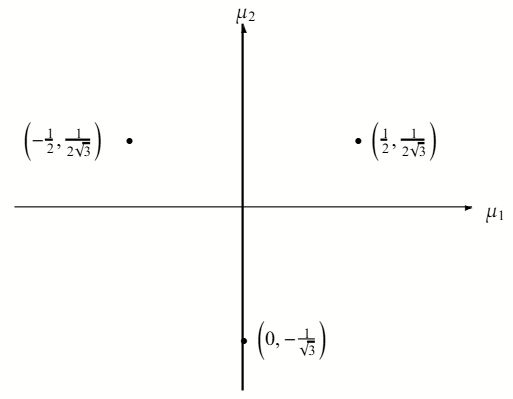
\includegraphics[width=0.44\linewidth]{Immagini - Capitolo 3/fundamental representation.png}
    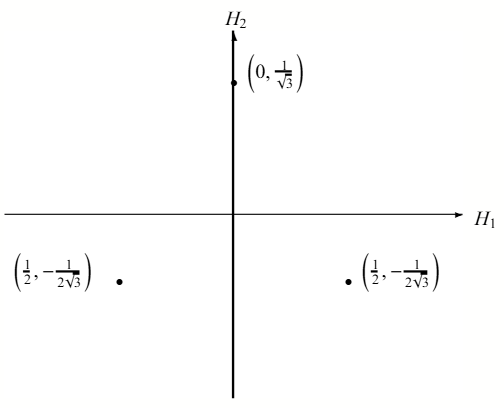
\includegraphics[width=0.42\linewidth]{Immagini - Capitolo 3/anti-fundamental representation.png}
    \caption{roots of the $\sua(3)$: (i) $\bm{3}$ fundamental representation; (ii) $\bar{\bm{3}}$ anti-fundamental representation.}
    \label{fig: fundamental and anti-fundamental representation of su(3)}
\end{figure}

In the defining representation of the $\sua(3)$ Lie algebra one can easily see that the highest weight $\ket{1/2,1/2\sqrt{3}}$ is not the lowest one $\ket{-1/2,1/2\sqrt{3}}$ with a minus sign. Thus, the $\sua(3)$ defining representation is a complex one. In Physics, it is customary to denote the defining representation as the ``fundamental representation'' and it is denoted by $\bm{3}$. Its complex conjugate representation is denoted ad $\bar{\bm{3}}$ and it is called the ``anti-fundamental representation'', with highest weight $\ket{1/2,-1/2\sqrt{3}}$; its weights are equal and opposite to those of the fundamental representation, and are shown again in figure \ref{fig: fundamental and anti-fundamental representation of su(3)}.

\section{Young diagrams for \texorpdfstring{$SU(N)$}{SU(N)}}
A generic irreducible representation $D$ of $SU(N)$ has the highest weight vector $\mu$, which can be expanded over the $N - 1$ fundamental weights $\mu^k$ as
\begin{equation}
    \mu = q^1\mu^1 + \cdots + q^{N-1}\mu^{N-1},
\end{equation}
so that alternatively one can specify $D$ with the Dynkin label $(q^1,\dots,q^{N-1})$. The irreducible representation $D$ can be associated with a Young diagram with $q^k$ columns of $k$ boxes, for $k = 1,\dots,N-1$, as shown below.
\ytableausetup{mathmode, boxframe=normal, boxsize=2.2em}
\begin{equation}
    \raisebox{8ex}{
        \begin{ytableau}
        1 & \cdots & \scriptstyle q^{N-1} & 1 & \cdots & 1 & \cdots & \scriptstyle q^2 & 1 & \cdots & \scriptstyle q^1 \\
        1 & \cdots & \scriptstyle q^{N-1} & 1 & \cdots & 1 & \cdots & \scriptstyle q^2 \\
        \none[\vdots] & \none[\vdots] & \none[\vdots] & \none[\vdots] & \none[\vdots] & \none[\vdots] \\
        1 & \cdots & \scriptstyle q^{N-1} & 1 & \cdots & \scriptstyle q^{N-2} \\
        1 & \cdots & \scriptstyle q^{N-1}
    \end{ytableau}
    }
\end{equation}
Alternatively, one could label the diagram by the number of boxes in each row; in the $k$th row there are $l_k$ boxes, with
\begin{equation}
    \begin{cases}
        l_1 = q^{N-1} + q^{N-2} + \cdots + q^2 + q^1 \\
        l_2 = q^{N-1} + q^{N-2} + \cdots + q^2 \\
        \vdots \\
        l_{N-1} = q^{N-1}
    \end{cases}.
\end{equation}
The table is now labelled by the list $\{l_1,\dots,l_{N-1}\}$, sometimes called the partition, resulting in the diagram below.
\begin{equation}
    \raisebox{0ex}{
        \begin{ytableau}
        1 & \cdots & \scriptstyle l_{N-1} & \cdots & \cdots & \scriptstyle l_{N-2} & \cdots & \scriptstyle l_3 & \cdots & \scriptstyle l_2 & \scriptstyle l_2 + 1 & \cdots & \scriptstyle l_1 \\
                1 & \cdots & \scriptstyle l_{N-1} & \cdots & \cdots & \scriptstyle \scriptstyle l_{N-2} & \cdots & \scriptstyle l_3 & \cdots & \scriptstyle l_2 \\
        \none[\vdots] & \none[\vdots] & \none[\vdots] & \none[\vdots] & \none[\vdots] & \none[\vdots] \\
        1 & \cdots & \scriptstyle l_{N-1} & \cdots & \cdots & \scriptstyle l_{N-2} \\
        1 & \cdots & \scriptstyle l_{N-1}
    \end{ytableau}
    }
\end{equation}
The dimension of the irreducible representation can be computed from its Young diagram using the factors-over-hooks rule. The rule works as follows. For an $\sua(N)$ diagram, put integers into boxes starting from the top-left corner, where the number $N$ is put. Then fill in the first row, increasing integers by one at each step to the right. For the second row, start from the left with $N - 1$, then fill the row, increasing the integers by one at each step. This goes on until all boxes in the diagram are filled. Then one computes the product of all the integers in the boxes, thus computing the number of factors, denoted as $F$. Moreover, a hook is a set of boxes with a shape like the $\neg$ symbol, that starts from the last box in a row, goes left and then turns down at some point, and continues down through the end of the column below. For each hook $i$, calculate the hook factor $h_i$, which is the number of boxes that the hook passes through. Then one calculates the product $H = \prod_ih_i$ over all hooks. The dimension of the representation is then the ratio
\begin{equation}
    \dim{D} = \frac{F}{H}.
\end{equation}
Consider now the tensor product of two irreducible representations $A \ot B$, using the corresponding Young diagrams. The process to compute this operation follows the general rules: 
\begin{enumerate}
    \item Put letters $a$ in the boxes on the first row of the diagram for $B$, letters $b$ in the second row, letters c in the third row, and so on, for example
    \begin{equation}
    \ytableausetup{mathmode, boxframe=normal, boxsize=1.3em}
    \raisebox{4ex}{
        \begin{ytableau}
        a & a & a & a \\
        b & b & b \\
        c \\
        d
        \end{ytableau}
        };
    \end{equation}
    \item take boxes with $a$ from $B$ and attach them in all possible ways to the ends of the rows of $A$ to get an expanded diagram, such that there is no more than one box with $a$ in each column of the expanded diagram $A$ (there can be more than one a per row);
    \item take the boxes with $b$ from $B$ and attach them to the previously obtained expanded diagram $A$, again enforcing that there is no more than one $b$ per column;
    \item take the boxes with $c$ from $B$ and attach them to the previously obtained expanded diagram $A$, again with the same rule, so that there is no more than one $c$ per column;
    \item repeat this procedure until all the letters have been used;
    \item for every diagram, form a word as follows: 
    \begin{enumerate}[i.]
        \item start reading the first row from right to left, at every step, add the letter that you encounter to the end of the word;
        \item after finishing the first row, move to the second row and repeat the process row by row and read from right to left adding letters to the word.
    \end{enumerate}
    \item generalize the previous definition of an admissible word if, by reading it from left to right, at every step at least as many $a$s have occurred as $b$s, $c$s, and so on, up to that point, at least as many $b$s have occurred as $c$s, $d$s, and so on, up to that point, and so on and so forth, for example $aabc$ and $ababc$ are admissible words, while $acba$ and $bca$ are not;
    \item discard the diagrams with non-admissible words, the remaining ones form the decomposition of the tensor product;
    \item identify every diagram as a $(q^1,\dots,q^{N-1})$ irreducible representation;
    \item compute their dimensions using the factors-over-hooks rule.
\end{enumerate}
\begin{ex}
    As an example, consider the decomposition of the tensor product of the adjoint representation $\bm{8}$ of the $\sua(3)$ algebra with itself, namely
    \begin{equation}
        \bm{8} \ot \bm{8} = \ydiagram{2,1} \ot \ytableaushort{aa,b}\,.
    \end{equation}
    So, following the rules, the first step leads to the diagrams
    \begin{equation}
        \ytableaushort{{}{}aa,{}}
        \,,\quad
        \ytableaushort{{}{}a,{}a}
        \,,\quad
        \ytableaushort{{}{}a,{},a}
        \,,\quad
        \ytableaushort{{}{},{}a,a}\,.
    \end{equation}
    Now, the process is repeated for the letter $b$, resulting in the diagrams
    \begin{gather}
        \cancel{\ytableaushort{{}{}aab,{}}}
        \,,\quad
        \ytableaushort{{}{}aa,{}b}
        \,,\quad
        \ytableaushort{{}{}aa,{},b}
        \,,\quad
        \cancel{\ytableaushort{{}{}ab,{}a}}
        \,, \\
        \ytableaushort{{}{}a,{}ab}
        \,,\quad
        \ytableaushort{{}{}a,{}a,b}
        \,,\quad
        \cancel{\ytableaushort{{}{}ab,{},a}}
        \,,\quad
        \ytableaushort{{}{}b,{}a,a}
        \,,\quad
        \ytableaushort{{}{},{}a,ab}
        \,.
    \end{gather}
    Thus, the decomposition is given by
    \begin{multline}
        \ytableaushort{{}{}aa,{}b} \op \ytableaushort{{}{}aa,{},b} \op \ytableaushort{{}{}a,{}ab} \op \ytableaushort{{}{}a,{}a,b}\, \op \\
        \op \ytableaushort{{}{}b,{}a,a} \op \ytableaushort{{}{},{}a,ab} = \ydiagram{4,2} \op \ydiagram{3}\, \op \\ \op \ydiagram{3,3} \op \ydiagram{2,1} \op \ydiagram{2,1} \op \bullet,
    \end{multline}
    or in a more compact notation
    \begin{multline}
        (2,2) \op (3,0) \op (0,3) \op (1,1) \op (1,1) \op (0,0) = \\ = \bm{27} \op \bm{10} \op \bar{\bm{10}} \op \bm{8} \op \bm{8} \op \bm{1}.
    \end{multline}
    Note that four diagrams were discarded with the non-admissible word $baa$ and were kept the six diagrams with the admissible words $aab$, $aab$, $aba$, $aab$, $aba$ and $aba$.
\end{ex}
\begin{ex}
    Consider the tensor product of the fundamental representation $\bm{3}$ with the antifundamental one $\bar{\bm{3}}$. Using again the set of rules for the product
    \begin{equation}
        \bm{3} \ot \bar{\bm{3}} = \ydiagram{1} \ot \ytableaushort{a,b}\,,
    \end{equation}
    gives two possibilities for the letter $a$, namely 
    \begin{equation}
        \ytableaushort{{}a}\,,\quad \ytableaushort{{},a}\,.
    \end{equation}
    Now, passing over to the letter $b$ the diagrams in the first case are
    \begin{equation}
        \cancel{\ytableaushort{{}{}ab}}\,,\quad \ytableaushort{{}a,b}\,,
    \end{equation}
    while in the second one are
    \begin{equation}
        \cancel{\ytableaushort{{}b,a}}\,,\quad \ytableaushort{{},a,b} = \ydiagram{2,1} \op \bullet.
    \end{equation}
    Thus, the decomposition is
    \begin{equation}
        \bm{3} \ot \bar{\bm{3}} = (1,1) \op (0,0) = \bm{8} \op \bm{1}.
    \end{equation}
    As a rule of thumb, it turns out that, in the $A \ot B$ product, it is generally convenient to take $B$ to be the representation with the simpler of the two Young diagrams; recall that, although the tensor product is not a commutative operation, $A \ot B$ and $B \ot A$ are equivalent up to a redefinition of the order of rows and columns, hence the two representations $A \ot B$ and $B \ot A$ are unitarily equivalent. In this regard, consider the tensor product $\bar{\bm{3}} \ot \bm{3}$, using the same rules on
    \begin{equation}
        \bar{\bm{3}} \ot \bm{3} = \ydiagram{1,1} \ot \ytableaushort{a}
    \end{equation}
    one has the diagrams
    \begin{equation}
        \ytableaushort{{}a,{}}\,,\quad \ytableaushort{{},{},a} = (1,1) \op (0,0),
    \end{equation}
    thus the decomposition, as expected, is the same found for the $\bm{3} \ot \bar{\bm{3}}$, namely $\bar{\bm{3}} \ot \bm{3} = \bm{8} \op \bm{1}$.
\end{ex}
\begin{ex}
    Consider the tensor product between the following two representations of the $\sua(4)$ algebra
    \begin{equation}
        \ydiagram{1,1} \ot \ytableaushort{a,b,c}\,,
    \end{equation}
    whose dimension is equal to 24 since the dimensions of the single representations, using the factors-over-hooks rule, are
    \begin{equation}
        \dim\left(\,\vcenter{\hbox{\ydiagram{1,1}}}\,\right) = 6,\quad \dim\left(\,\vcenter{\hbox{\ydiagram{1,1,1}}}\,\right) = 4.
    \end{equation}
    For the first letter there are only two possibilities
    \begin{equation}
        \ytableaushort{{}a,{}}\,,\quad \ytableaushort{{},{},a}\,.
    \end{equation}
    Passing over to the second letter $b$ the number of diagrams grows to
    \begin{equation}
        \ytableaushort{{}ab,{}}\,,\quad \ytableaushort{{}a,{}b}\,,\quad \ytableaushort{{}a,{},b}\,,\quad \ytableaushort{{}b,{},a}\,,\quad \ytableaushort{{},{},a,b}\,.
    \end{equation}
    Then, considering the last letter, the total number of diagrams consist in
    \begin{gather}
        \ytableaushort{{}ab,{}c}\,,\quad \ytableaushort{{}abc,{}}\,,\quad \ytableaushort{{}ab,{},c}\,,\quad \ytableaushort{{}ac,{}b}\,,\quad \ytableaushort{{}a,{}b,c} \\
        \ytableaushort{{}ac,{}b}\,,\quad \ytableaushort{{}a,{},b,c}\,,\quad \ytableaushort{{}bc,{},a}\,,\quad \ytableaushort{{}c,{},a,b}\,,\quad \ytableaushort{{},{},a,b,c}\,.
    \end{gather}
    Now removing the non-admissible diagrams the tensor product in question results in 
    \begin{equation}
        \ydiagram{1,1} \ot \ydiagram{1,1,1} = \ydiagram{2,2,1} \op \ydiagram{2,1,1,1} = \ydiagram{2,2,1} \op \ydiagram{1}\,.
    \end{equation}
    To check if the tensor product result is coherent, one can compute the dimensions of the diagrams obtained, which in this case are
    \begin{equation}
        \dim\left(\,\vcenter{\hbox{\ydiagram{2,2,1}}}\,\right) = 20,\quad \dim\left(\,\vcenter{\hbox{\ydiagram{1}}}\,\right) = 4,
    \end{equation}
    whose sum is 24 as expected.
\end{ex}

\section{Lorentz group}
The Lorentz group is the group of transformations of spacetime coordinate in special relativity relating quantities measured by different observers in motion at constant speed with respect to each other, in other words by observers in different inertial frames of reference. Special relativity is based on two postulates:
\begin{enumerate}
    \item all physical laws have the same form in all inertial frames;
    \item the speed of light in a vacuum is the same in all inertial frames.
\end{enumerate}
Consider two inertial reference frames with spacetime coordinates $x^\mu = (t,x^1,x^2,x^3)$ and $x'^\mu = (t,x'^1,x'^2,x'^3)$ and assume that at $t = t' = 0$ the two frames coincide, namely $x^\mu(t = 0) = x'^\mu(t' = 0)$. Then, according to the second postulate of special relativity, a ray of light emitted at the origin at that time ans propagating to another point $P$ at a later time should be such that the spacetime coordinated of $P$ measured in the two inertial frames satisfy
\begin{equation}
    (ct)^2 - x_ix^i = (ct')^2 - x_i'x'^i.
\end{equation}
Introducing the Minkowski metric $g_{\mu\nu}$ as the matrix\footnote{One can also define the Minkowski metric as $g_{\mu\nu} = \mathrm{diag}(-1,1,1,1)$, which is often used in spacial and general relativity, but usually the convention in particle physics is given by equation \eqref{eq: Minkowski metric definition}; either way the results obtained through them are equivalent.}
\begin{equation}
\label{eq: Minkowski metric definition}
    g_{\mu\nu} = 
    \begin{pmatrix}
        1 & 0 & 0 & 0 \\
        0 & - 1 & 0 & 0 \\
        0 & 0 & -1 & 0 \\
        0 & 0 & 0 & -1
    \end{pmatrix},
\end{equation}
the latter equation can be written as
\begin{equation}
\label{eq: invariance of relativistic interval}
    g_{\mu\nu}x^\mu x^\nu = g_{\mu\nu}x'^\mu x'^\nu.
\end{equation}
In special relativity, an event is defined as a point in spacetime, so given two events $A$ and $B$, on can define the squared relativistic interval $\Delta s_{AB}^2$ as
\begin{equation}
    \Delta s_{AB}^2 = (x_A^0 - x_B^0)^2 - (x_A^i - x_B^i)^2 = g_{\mu\nu}(x_A - x_B)^\mu(x_A - x_B)^\nu,
\end{equation}
and this quantity is an example of a relativistic invariant, namely a quantity that has the property to have the same value in all inertial frames. Assuming that the spacetime coordinates of an event expressed in two different inertial frames, $x^\alpha$ and $x^\beta$, are related to each other by a set of linear transformations
\begin{equation}
\label{eq: Lorentz transformation}
    x'^\beta = \Lambda^\beta_\alpha x^\alpha.
\end{equation}
Furthermore, equation \eqref{eq: invariance of relativistic interval} implies that 
\begin{equation}
    g_{\mu\nu}x^\mu x^\nu = g_{\alpha\beta}\Lambda^\alpha_\mu \Lambda^\nu_\beta x^\mu x^\nu,
\end{equation}
and since this must hold for every arbitrary $x^\mu$ it follows that
\begin{equation}
\label{eq: RS principle}
    g_{\mu\nu} = g_{\alpha\beta}\Lambda^\alpha_\mu \Lambda^\nu_\beta.
\end{equation}
A spacetime coordinate transformation $\Lambda$ which satisfies equation \eqref{eq: RS principle} is called a Lorentz transformation. Consider the $\mu = \nu = 0$ component of again equation \eqref{eq: RS principle}, that is 
\begin{equation}
    1 = g_{\alpha\beta}\Lambda^\alpha_0 \Lambda^\nu_0 = (\Lambda_0^0)^2 - (\Lambda_0^i)^2,
\end{equation}
from which one deduces that
\begin{equation}
    |\Lambda^0_0| = \sqrt{1 + (\Lambda_0^i)^2} \ge 1.
\end{equation}
Depending on the sign of $\Lambda_0^0$, the transformation represented by the $\Lambda$ matrix is said to be:
\begin{enumerate}
    \item an orthochronous Lorentz transformation if $\Lambda_0^0 \ge 1$;
    \item an antichronous Lorentz transformation if $\Lambda_0^0 \le -1$.
\end{enumerate}
Moreover, if one interprets $x^\mu$ and $x'^\mu$ coordinates as four-component, real-valued column vectors, and $g$ and $\Lambda$ as $4 \times 4$ real-valued matrices, then equation \eqref{eq: RS principle} can be thought of as the matrix relation 
\begin{equation}
\label{eq: RS principle in matrix form}
    g = \Lambda^Tg\Lambda.
\end{equation}
Taking the determinant of equation \eqref{eq: RS principle in matrix form}, one deduces that $\det{\Lambda} = \pm1$. Accordingly, one distinguishes:
\begin{enumerate}
    \item a proper Lorentz transformation if $\det{\Lambda} = 1$;
    \item an improper Lorentz transformation if $\det{\Lambda} = -1$;
\end{enumerate}
One can note that equation \eqref{eq: RS principle in matrix form} has an analogy with the one that characterises the group of orthogonal transformation of size four, denoted as $O(4)$, namely $\MI_4 = O^T\MI_4O$, the difference being that $\MI_{\mu\nu} = \delta_{\mu\nu}$ while $g_{\mu\nu}$ is defined as in equation \eqref{eq: Minkowski metric definition}. To stress the fact that three diagonal entries of $g_{\mu\nu}$ have the same sign, while one has the opposite sign, the set of matrices satisfying equation \eqref{eq: RS principle in matrix form} is denoted as $O(3,1)$. These matrices, with the matrix row-by-column multiplication as the group product, form a group called the Lorentz group. This group can be defined as the set of coordinate transformation leaving the $\Delta s^2$ invariant. Furthermore, while $x_\mu x^\mu$ is always non-negative and it is zero if and only if $x^\mu = 0$, the invariant $\Delta s^2$ can be either positive, zero or negative. Accordingly, a four-vector $x^\mu$ is said to be:
\begin{enumerate}
    \item a timelike four-vector if $(x^0)^2 - (x^i)^2 > 0$;
    \item a lightlike four-vector if $(x^0)^2 - (x^i)^2 = 0$;
    \item a spacelike four-vector if $(x^0)^2 - (x^i)^2 < 0$.
\end{enumerate}

\subsubsection{Rotations}
Matrices of the form 
\begin{equation}
\label{eq: general Lorentz rotation}
    \Lambda = 
    \begin{pmatrix}
        1 & 0 & 0 & 0 \\
        0 & & & \\
        0 & & R & \\
        0 & & &
    \end{pmatrix},\quad R \in O(3),
\end{equation}
describe transformations that leave the $x^0$ coordinate unchanged, and rotate the spatial axes of the reference frames; the transformation is an orthochronus Lorentz transformation and it is proper if $\det{R} = 1$, namely if $R \in SO(3)$. Note that the inverse transformation $\Lambda^{-1}$ has the same for as $\Lambda$, but with $R$ replaced with $R^T$. 

As a particular case of equation \eqref{eq: general Lorentz rotation}, a rotation of the reference frame by an angle $\theta$ around the $z$-axis takes the form 
\begin{equation}
    \Lambda =
    \begin{pmatrix}
        1 & 0 & 0 & 0 \\
        0 & \cos{\theta} & \sin{\theta} & 0 \\
        0 & -\sin{\theta} & \cos{\theta} & 0 \\
        0 & 0 & 0 & 1
    \end{pmatrix}.
\end{equation}
When the angle $\theta$ is infinitesimally small, one can expand around the unit element
\begin{equation}
    \Lambda =
    \begin{pmatrix}
        1 & 0 & 0 & 0 \\
        0 & 1 & \theta & 0 \\
        0 & -\theta & 1 & 0 \\
        0 & 0 & 0 & 1
    \end{pmatrix} = \MI_4 +i\theta
    \begin{pmatrix}
        0 & 0 & 0 & 0 \\
        0 & 0 & -i & 0 \\
        0 & i & 0 & 0 \\
        0 & 0 & 0 & 0
    \end{pmatrix} + o(\theta^2)
\end{equation}
from which one can read off the generator of rotations around the $z$-axis as the matrix multiplied by $i\theta$ in the last term. With a similar argument, one can derive the generators of rotations around the other two spatial axes, finding
\begin{equation}
    J^1 = 
    \begin{pmatrix}
        0 & 0 & 0 & 0 \\
        0 & 0 & 0 & 0 \\
        0 & 0 & 0 & -i \\
        0 & 0 & i & 0
    \end{pmatrix},\quad
    J^2 = 
    \begin{pmatrix}
        0 & 0 & 0 & 0 \\
        0 & 0 & 0 & i \\
        0 & 0 & 0 & 0 \\
        0 &-i & 0 & 0
    \end{pmatrix},\quad
    J^3 = 
    \begin{pmatrix}
        0 & 0 & 0 & 0 \\
        0 & 0 & -i & 0 \\
        0 & i & 0 & 0 \\
        0 & 0 & 0 & 0
    \end{pmatrix}
\end{equation}
which form an $\sua(2)$ algebra since they satisfy the commutation relation
\begin{equation}
    \comm{J^a}{J^b} = i\epsilon_{abc}J^c.
\end{equation}

Another particular case of equation \eqref{eq: general Lorentz rotation} is the parity transformation, namely the inversion of all spatial coordinates, corresponding to imposing $R = -\MI_3$ in said equation, which is a improper orthochronus Lorentz transformation. Note that the parity transformation does not depend on a continuous parameter, because of that it is a discrete transformation. Furthermore, parity transformation is such that its square equals the identity, hence it is equal to its inverse.

\subsubsection{Boosts}
Relativistic transformations of the spacetime coordinates between two inertial reference frames moving at constant relative velocity of modulus $v$ are called Lorentz boosts; in the particular case where the reference frame with coordinates $x'^\mu$ is moving with respect to the reference frame with coordinates $x^\mu$ at velocity $v$ along the $x$-direction then the boost can be represented by the matrix
\begin{equation}
    \Lambda = 
    \begin{pmatrix}
        \gamma & -\beta\gamma & 0 & 0 \\
        -\beta\gamma & \gamma & 0 & 0 \\
        0 & 0 & 0 & 0 \\
        0 & 0 & 0 & 0
    \end{pmatrix},
\end{equation}
that by defining the rapidity $\eta = \arcsinh{(\beta\gamma)}$ can be also written as
\begin{equation}
\label{eq: Lorentz boost along x-axis (rapidity)}
    \Lambda = 
    \begin{pmatrix}
        \cosh{\eta} & -\sinh{\eta} & 0 & 0 \\
        -\sinh{\eta} & \cosh{\eta} & 0 & 0 \\
        0 & 0 & 1 & 0 \\
        0 & 0 & 0 & 1
    \end{pmatrix}.
\end{equation}
In order to give a proper definition of infinitesimal boosts, recall first that the condition that defines a Lorentz transformation is $g_{\mu\nu} = g_{\alpha\beta}\Lambda^\alpha_\mu\Lambda^\beta_\nu = \Lambda_{\beta\mu}\Lambda^\beta_\nu$; when $\Lambda$ is a proper and orthochronus Lorentz trasformation infinitesimally close to the identity, one can write
\begin{equation}
    \Lambda^\alpha_\mu = g^\alpha_\mu + \omega^\alpha_\mu,
\end{equation}
where the components of $\omega$ are infinitesimally small, so that one has
\begin{equation}
    g_{\mu\nu} = \Lambda_{\beta\mu}\Lambda^\beta_\nu \simeq (g_{\beta\mu} + \omega_{\beta\mu})(g^\beta_\nu + \omega^\beta_\nu) = g_{\mu\nu} + \omega_{\mu\nu} + \omega_{\nu\mu},
\end{equation}
from which the following condition is obtained
\begin{equation}
    \omega_{\mu\nu} = - \omega_{\nu\mu}.
\end{equation}
Now, consider again the matrix in equation \eqref{eq: Lorentz boost along x-axis (rapidity)} in the limit where $\eta$ is infinitesimally small, then
\begin{equation}
    \Lambda = 
    \begin{pmatrix}
        1 & -\eta & 0 & 0 \\
        -\eta & 1 & 0 & 0 \\
        0 & 0 & 1 & 0 \\
        0 & 0 & 0 & 1 \\
    \end{pmatrix} = \MI_4 + i\eta
    \begin{pmatrix}
        0 & i & 0 & 0 \\
        i & 0 & 0 & 0 \\
        0 & 0 & 0 & 0 \\
        0 & 0 & 0 & 0 \\
    \end{pmatrix} + o(\eta^2)
\end{equation}
from which one can read off the generator of Lorentz boosts along the $x$-axis as the matrix multiplied by the $i\eta$ in the last term. With a similar argument, one can derive the generators of Lorentz boosts along the other two spatial axes, finding 
\begin{equation}
    K^1 = 
    \begin{pmatrix}
        0 & i & 0 & 0 \\
        i & 0 & 0 & 0 \\
        0 & 0 & 0 & 0 \\
        0 & 0 & 0 & 0
    \end{pmatrix},\quad
    K^2 = 
    \begin{pmatrix}
        0 & 0 & i & 0 \\
        0 & 0 & 0 & 0 \\
        i & 0 & 0 & 0 \\
        0 & 0 & 0 & 0
    \end{pmatrix},\quad
    K^3 = 
    \begin{pmatrix}
        0 & 0 & 0 & i \\
        0 & 0 & 0 & 0 \\
        0 & 0 & 0 & 0 \\
        i & 0 & 0 & 0
    \end{pmatrix}.
\end{equation}
Note that the $K^a$ generators are anti-Hermitian. Anyway, in contrast to the generators of rotations, the boosts generators do not form a closed subalgebra themselves; instead
\begin{equation}
\label{eq: commutator between K and K}
    \comm{K^a}{K^b} = -i\epsilon_{abc}J^c.
\end{equation}
Moreover, the commutator of a rotation generator and a boost generator reads
\begin{equation}
\label{eq: commutator between J and K}
    \comm{J^a}{K^b} = i\epsilon_{abc}K^c.
\end{equation}

\subsubsection{Time inversion}
The Lorentz transformation described by the matrix 
\begin{equation}
    \Lambda = 
    \begin{pmatrix}
        -1 & 0 & 0 & 0 \\
        0 & 1 & 0 & 0 \\
        0 & 0 & 1 & 0 \\
        0 & 0 & 0 & 1
    \end{pmatrix}
\end{equation}
is an improper non-orthochronus Lorentz transformation that reverses the sign of time, leaving the spatial coordinates, as well as the $\Delta s^2$ invariant, unchanged. Like the parity transformation, the time inversion is a discrete transformation which squares the identity and, hence, equals its inverse.

\subsection{Lorentz group algebra}
While the relations \eqref{eq: commutator between K and K} and \eqref{eq: commutator between J and K} imply that generators of rotations and the generators of boosts do not form separate algebras, one can prove that, defining the following combinations of generators 
\begin{equation}
    N^a = \frac{1}{2}(J^a + iK^a),\quad M^a = \frac{1}{2}(J^a - iK^a),
\end{equation}
one obtains the two independent $\sua(2)$ algebras
\begin{equation}
    \comm{N^a}{N^b} = i\epsilon_{abc}N^c,\quad \comm{M^a}{M^b} = i\epsilon_{abc}M^c,\quad \comm{N^a}{M^b} = 0.
\end{equation}
Accordingly, the irreducible representations of the Lorentz group can be labelled by the labels of these two $\sua(2)$ subalgebras $(p,q)$ where $p$ and $q$ are integers or half-integers non-negative numbers related to the quadratic Casimir operator constructed from the $N^a$ and the $M^a$ generators as
\begin{equation}
    N_aN^a = p(p + 1)\MI_4,\quad M_aM^a = q(q + 1)\MI_4.
\end{equation}
Restrict now the discussion to the subset of continuos proper orthochronus Lorentz transformations, namely rotations and boosts. As discussed previously, they depend on six parameters, in particular three rotation angles and three components of the boost velocity. Consider then a Lorentz transformation that is infinitesimally close to the identity
\begin{equation}
\label{eq: infinitesimal Lorentz transformation}
    \Lambda^\beta_\alpha = \delta^\beta_\alpha + \epsilon^\beta_\alpha + o(\epsilon^2),
\end{equation}
that substituted in equation \eqref{eq: RS principle} gives
\begin{equation}
    \begin{split}
        g_{\mu\nu} &= g_{\alpha\beta}[\delta^\beta_\mu + \epsilon^\beta_\mu + o(\epsilon^2)][\delta^\beta_\nu + \epsilon^\beta_\nu + o(\epsilon^2)] \\
        &= g_{\alpha\beta}[\delta^\alpha_\mu\delta^\beta_\nu + \epsilon^\alpha_\mu\delta^\beta_\nu + \delta^\alpha_\mu\epsilon^\beta_\nu + o(\epsilon^2)] \\
        &= g_{\mu\nu} + \epsilon_{\nu\mu} + \epsilon_{\mu\nu} + o(\epsilon^2),
    \end{split}
\end{equation}
from which it follows the above found relation $\epsilon_{\mu\nu} = -\epsilon_{\nu\mu}$, implying that the infinitesimal generator of Lorentz transformations can be thought of as an antisymmetric $4 \times 4$ tensor with six independent components. Consider now the differential operator defined as
\begin{equation}
    L_{\mu\nu} = ix_\mu\frac{\p}{\p x^\nu} - ix_\nu\frac{\p}{\p x^\mu} \equiv i(x_\mu\p_\nu - x_\nu\p_\mu),
\end{equation}
they satisfy the Lorentz algebra
\begin{equation}
    \comm{L^{\alpha\beta}}{L^{\gamma\delta}} = i(g^{\beta\gamma}L^{\alpha\delta} + g^{\alpha\delta}L^{\beta\gamma} - g^{\beta\delta}L^{\alpha\gamma} - g^{\alpha\gamma}L^{\beta\delta})
\end{equation}
and allow one to write the variation of $x^\nu$ under an infinitesimal Lorentz transformation as
\begin{equation}
    \delta x^\nu = \frac{i}{2}\epsilon^{\alpha\beta}L_{\alpha\beta} x^\nu.
\end{equation}
For a Lorentz transformation that can be expressed as in equation \eqref{eq: infinitesimal Lorentz transformation}, one can thus define the operator
\begin{equation}
    U(\Lambda) = \exp{\bigg(\frac{i}{2}\epsilon^{\alpha\beta}L_{\alpha\beta}\bigg)},
\end{equation}
which can be used to classify the different type of fields based on their transformation properties under a Lorentz transformation. These transformations properties must account for the nature of the field and for the fact that it depends on spacetime coordinates which are not invariant under Lorentz transformations; for example, a scalar field $\phi(x)$ transforms as
\begin{equation}
    \phi(x') = U(\Lambda)\phi(x)U^{-1}(\Lambda),
\end{equation}
while a vector field $\phi^\alpha(x)$ transforms as
\begin{equation}
    \phi^\beta(x') = \Lambda^\beta_\alpha[U(\Lambda)\phi^\alpha(x)U^{-1}(\Lambda)].
\end{equation}
In fact, there could be many more types of fields, which could be constructed, for example, by considering the representation of the $\sua(2)$ algebras generated by the $N^a$and $N^{a\dg}$, that one can denote as $\bm{(p,q)}$, and their product. For instance:
\begin{enumerate}
    \item $\bm{(0,0)}$ corresponds to a scalar field;
    \item $\bm{(1/2,0)}$ corresponds to a left-handed, spin-half field;
    \item $\bm{(0,1/2)}$ corresponds to a right-handed, spin-half field;
    \item the product $\bm{(1/2,0)} \ot \bm{(0,1/2)} = \bm{(1/2,1/2)}$ corresponds to a spin-one vector field;
    \item the product $\bm{(1/2,0)} \ot \bm{(1/2,0)} = \bm{(0,0)} \op \bm{(1,0)}$ corresponds to a scalar representation times a two-index, antisymmetric, self-dual tensor;
    \item the product $\bm{(0,1/2)} \ot \bm{(0,1/2)} = \bm{(0,0)} \op \bm{(0,1)}$ corresponds to a scalar representation times a two-index, antisymmetric, anti-self-dual tensor.
\end{enumerate}
\begin{obs}
    The field strength tensor of electromagnetism is a physical example of a field transforming in the $\bm{(1,0)} \op \bm{(0,1)}$ representation of the Lorentz group.
\end{obs}

\section{Lorentz-Poincaré group}
As discussed above, the Lorentz group consists of the linear coordinate transformation that are consistent with the principles of special relativity theory. However, as the physical laws depend only on differences of physical coordinates, one can extend the set of coordinate transformations to include also spacetime translations, generalising equation \eqref{eq: Lorentz transformation} to
\begin{equation}
\label{eq: Lorentz-Poincaré transformation}
    x'^\beta = \Lambda^\beta_\alpha x^\alpha + a^\beta,
\end{equation}
where $a^\beta$ is a constant four-vector. The transformations defined in equation \eqref{eq: Lorentz-Poincaré transformation} can be concisely denoted as $(\Lambda,a)$ and form the Lorentz-Poincaré group, which is a ten-dimensional group. The group product of two generic elements $(\Lambda_1,a_1)$ and $(\Lambda_2,a_2)$ of the Lorentz-Poincaré group can be evaluated by writing first $x' = \Lambda_2x + a_2$, then $x'' = \Lambda_1x_1' + a_1$, from which one deduces $x'' = \Lambda_1\Lambda_2x + \Lambda_1a_2 + a_1$. Hence, the group product for the Lorentz-Poincaré group is given by
\begin{equation}
    (\Lambda_1,a_1) \cdot (\Lambda_2,a_2) = (\Lambda_1\Lambda_2, \Lambda_1a_2 + a_1).
\end{equation}
For this reason, the Lorentz-Poincaré product is said to be the semi-direct product of the Lorentz group and the group of translations. 

The generators of the Lorentz-Poincaré group include six generators of the Lorentz group $L^{\alpha\beta}$, and the four generators of translations $P^\alpha$. They satisfy the commutation relation
\begin{equation}
    \begin{cases}
        \comm{L^{\alpha\beta}}{L^{\gamma\delta}} = i(g^{\beta\gamma}L^{\alpha\delta} + g^{\alpha\delta}L^{\beta\gamma} - g^{\beta\delta}L^{\alpha\gamma} - g^{\alpha\gamma}L^{\beta\delta}) \\
        \comm{L^{\alpha\beta}}{P^\gamma} = i(g^{\alpha\gamma}P^\beta - g^{\beta\gamma}P^\alpha) \\
        \comm{P^\alpha}{P^\beta} = 0
    \end{cases}.
\end{equation}
The Lorentz-Poincaré group has two Casimir operators:
\begin{enumerate}
    \item $P_\alpha P^\alpha$, which in the context of quantum field theory, where $P^\alpha$'s components of the four-momentum of a particle, its eigenvalue is nothing but the squared mass of the particle, namely
    \begin{equation}
        P_\alpha P^\alpha = m^2\MI_4;
    \end{equation}
    \item $W_\alpha W^\alpha$, where $W^\alpha$ is the Pauli-Lubanski axial vector defined as
    \begin{equation}
        W^\alpha = \frac{1}{2}\epsilon^{\alpha\beta\gamma\delta}P_\beta L_{\beta\gamma},
    \end{equation}
    whose eigenvalue is the squared product between the mass and he angular momentum of the particle, namely
    \begin{equation}
        W_\alpha W^\alpha = -m^2J(J + 1),
    \end{equation}
    where $J$ is a non-negative integer or a half-integer; in particular, for massive particles, the number of physical states is $2J + 1$, while for massless particles, the Pauli-Lubanski axial vector is proportional to the momentum four-vector $W_\alpha = hP_\alpha$ where $h = \pm J$ is the helicity of the particle, and there are two physical states.
\end{enumerate}
Finally, note that both the Lorentz group and the Lorentz-Poincaré group are non-compact. 

